\documentclass[11pt,oneside]{book}

\usepackage[a4paper,margin=2.5cm]{geometry}
\usepackage{xcolor}
\usepackage{amsmath}
\usepackage{microtype}
\usepackage{graphicx}
\usepackage{booktabs}
\usepackage{hyperref}
\usepackage[most]{tcolorbox}

\graphicspath{{../../results/plots/}{results/plots/}}

\definecolor{todofill}{HTML}{FFF3CD}
\definecolor{todotext}{HTML}{7A5200}
\definecolor{pendingfill}{HTML}{EEF3FB}
\definecolor{pendingline}{HTML}{B3C6E0}
\definecolor{pendingtext}{HTML}{34568B}

\hypersetup{
  colorlinks=true,
  linkcolor=pendingtext,
  citecolor=pendingtext,
  urlcolor=pendingtext,
  pdftitle={Memory Pruning and Forgetting Policies for AI Coding Agents}
}

\newtcolorbox{todobox}{
  colback=todofill,
  colframe=todofill,
  coltext=todotext,
  boxrule=0pt,
  arc=2pt,
  left=7pt,
  right=7pt,
  top=7pt,
  bottom=7pt,
  before upper={\textbf{TODO \textperiodcentered{}}\ },
}

\newtcolorbox{figurestub}[2][]{
  colback=pendingfill,
  colframe=pendingline,
  coltext=pendingtext,
  arc=3pt,
  title={\textbf{[PENDING] #2}},
  fonttitle=\normalsize,
  #1
}

\setlength{\parindent}{1.5em}
\setlength{\parskip}{0.25em}
\linespread{1.08}


\title{Memory Pruning and Forgetting Policies for AI Coding Agents\\
\large Impact on Performance Across Sequential Tasks}
\author{}
\date{Master's Thesis}

\begin{document}

\frontmatter
\begin{titlepage}
  \centering
  \vspace*{2.5cm}
  {\LARGE\bfseries Memory Pruning and Forgetting Policies\\
   for AI Coding Agents\par}
  \vspace{0.6em}
  {\large Impact on Performance Across Sequential Tasks\par}
  \vspace{2.5cm}
  {\large A thesis submitted in partial fulfillment\\
   of the requirements for the degree of\\
   Master of Science\par}
  \vspace{2cm}
  {\large\itshape \textcolor{gray}{[Author Name]}\par}
  \vspace{0.5em}
  {\normalsize \textcolor{gray}{[Department, University]}\par}
  \vspace{0.4em}
  {\normalsize Supervisor: \textcolor{gray}{[Supervisor Name]}\par}
  \vfill
  {\normalsize \today\par}
\end{titlepage}

% Generated from the matching Typst scaffold by
% scripts/migrate_typst_report_to_latex.py (prose drafted 2026-06-25).
% INTEGRITY: model = deepseek-v4-flash. The RESULTS clause must NOT assert the pending
% headline -- it states the question; the finding is [RESULT: pending runs_144_seq_cceb325].
% No TOST claim. Thread "retrieval held constant", "non-inferiority", "footprint".

% ── Abstract ─────────────────────────────────────────────────────────────
% PURPOSE: 130-160-word structured abstract of the whole thesis.
% ─────────────────────────────────────────────────────────────────────────

\chapter*{Abstract}\addcontentsline{toc}{chapter}{Abstract}

LLM coding agents resolve real repository issues, but applying them across long
\emph{sequences} of related tasks is harder: experience accumulates as persistent memory, yet
naive accumulation inflates cost with no proven benefit and can even mislead. Rather than
invent another memory policy, we isolate \emph{storage} from \emph{retrieval}: six forgetting
policies, bracketed by No Memory and Full Memory, are compared under \emph{identical,
retrieval-held-constant} cosine search, a single frozen model (\texttt{deepseek-v4-flash}),
and a 144-run matrix over the eight SWE-Bench-CL sequences and three seeds. The analysis is
pre-registered and effect-size-first (Wilcoxon on $N=8$ sequence means, rank-biserial effect
sizes, bootstrap intervals), with cost read on two axes, compute and memory footprint. We ask
whether proactive forgetting is non-inferior to full accumulation, and at what footprint:
\texttt{[RESULT: pending runs\_144\_seq\_cceb325]}. The contribution is a controlled
\emph{measurement} --- including an instrument-validation sub-study that caught and fixed a
tooling defect before the matrix --- of \emph{when} and \emph{how much} a coding agent should
forget, not a new policy.

\clearpage
\tableofcontents\clearpage
\listoffigures\clearpage
\listoftables\clearpage

\mainmatter
\chapter{Introduction}\label{ch:intro}
% Generated from the matching Typst scaffold by
% scripts/migrate_typst_report_to_latex.py (prose drafted 2026-06-25).

% ── 1.1  Background and Motivation ──────────────────────────────────────────
% PURPOSE: Motivate persistent memory for LLM coding agents on long-horizon work.
% MOVE: Scale+stakes -> traditional approach -> structural limitation.
% ─────────────────────────────────────────────────────────────────────────

\section{Background and Motivation}

Large language model (LLM) coding agents have entered the SWE-Bench era: given a
natural-language issue and a real repository, an agent now plans, edits files, runs the
test suite, and iterates until the issue is resolved, autonomously and end to
end~\cite{joshi2025}. The capability is no longer a laboratory curiosity --- agents
resolve a non-trivial fraction of genuine GitHub issues drawn from mature open-source
projects --- and the stakes scale with it: the same automation that closes one issue is
expected to work an entire backlog.

Real software-engineering work, however, is rarely a sequence of isolated one-shot
prompts. It is long-horizon and \emph{sequential}: many related tasks accrue over the
lifetime of a single codebase, each leaving behind a diagnosis, a fix, and a lesson that
might inform the next. An agent that treats every issue as if it were the first throws
away precisely the experience a human maintainer would carry forward. The natural remedy
is to externalise that experience as \emph{persistent memory} --- a store of past
problems and their solutions that the agent can consult on future
tasks~\cite{packer2024,zhong2024}. This is the premise behind a growing family of agent
memory systems, and it is intuitively compelling: an agent that remembers more of its
past should solve more of its future.

The traditional way to operationalise that premise is simply to keep everything. Each
completed task appends a record; nothing is ever discarded. But naive accumulation has a
structural cost. Context windows are finite and, more importantly, they are not free to
fill: longer prompts raise token cost and latency, and a well-documented body of evidence
shows that model performance degrades as relevant information is buried among
distractors~\cite{liu2024} and even as raw context length grows with retrieval held
perfect~\cite{du2025}. Worse, more memory is not merely more expensive --- it can be
actively harmful. Recent empirical work shows that agents exhibit
\emph{experience-following}, faithfully reusing retrieved precedents even when those
precedents mislead, so that a larger or lower-quality memory store degrades
behaviour rather than improving it~\cite{xiong2025}.

This sets up the structural limitation that motivates the thesis. If keeping everything is
costly and sometimes harmful, then an agent ought to forget --- but \emph{forgetting} is
itself a policy decision with no obvious right answer, and it is entangled with how memory
is retrieved. Does retained experience actually help downstream coding performance, or does
it mostly inflate the prompt? And if some forgetting is warranted, \emph{when} and
\emph{how much}? These questions have been asked for conversational and
general-purpose agents, but they have not been answered cleanly for coding agents under a
controlled comparison. Figure~\ref{fig:architecture} situates the question: storage and
forgetting are one component in a pipeline that also includes retrieval, and only by
holding the rest fixed can the effect of forgetting be read off in isolation.

% Generated from the matching Typst scaffold by
% scripts/migrate_typst_report_to_latex.py.

% ── 1.2  Problem Statement ──────────────────────────────────────────────────
% PURPOSE: Name the pain, its consequence, and the unmet research gap.
% MOVE: Pain → Consequence → Gap ("therefore there exists a need …").
% BEATS: pain (bloat vs lossy pruning) · consequence (cost + entanglement) · gap.
% FIGURES/TABLES: none.
% CITATIONS: xiong2025 (more memory can hurt — experience-following),
%            alqithami2025 (closest six-policy prior — NOVELTY-THREAT).
% ─────────────────────────────────────────────────────────────────────────

\section{Problem Statement}

\begin{todobox}
Expand the beats below using Pain \textrightarrow{} Consequence \textrightarrow{} Gap, ending on an explicit "therefore there exists a need …". Pre-empt Alqithami (alqithami2025) as a novelty threat: conversational domain, retrieval not isolated.
\end{todobox}

% - PAIN: full memory bloats the context window; but naive pruning may drop
%   task-critical knowledge — both failure modes are real.
% - more memory can actively hurt via experience-following / interference,
%   not merely cost @xiong2025.
% - CONSEQUENCE: cost and latency rise with accumulation; worse, prior work
%   *entangles* the storage (forgetting) policy with the retrieval policy, so
%   no benefit is cleanly attributable — and none is demonstrated on coding.
% - NOVELTY-THREAT: @alqithami2025 is the closest six-policy comparison, but it
%   is conversational and does *not* hold retrieval constant — differentiate now.
% - GAP (therefore): there exists no controlled, *retrieval-fixed* comparison of
%   forgetting policies for coding agents — the central control this thesis adds.

% Generated from the matching Typst scaffold by
% scripts/migrate_typst_report_to_latex.py (prose drafted 2026-06-25).

% ── 1.3  Research Questions and Scope ───────────────────────────────────────
% PURPOSE: State the central RQ, sub-questions, and the (anti-creep) scope.
% MOVE: Operational-narrative objectives (primary -> secondary -> constraint).
% ─────────────────────────────────────────────────────────────────────────

\section{Research Questions and Scope}

The central research question is whether proactive forgetting and consolidation policies
can match the task-resolution performance of full-memory accumulation at materially lower
cost, and --- if any difference exists --- which \emph{content-aware} structure of
forgetting matters most. The framing throughout is that \emph{not every task needs
memory}: the question is not how to remember more, but when and how much to forget without
paying for it in resolved issues. We instantiate the question on the SWE-Bench-CL
continual-learning benchmark for coding agents~\cite{joshi2025}.

This primary question decomposes into five secondary questions, in descending order of
how load-bearing they are for the thesis:

\begin{itemize}
  \item \textbf{SQ1 (trade-off).} How do the six policies compare on continual-learning
        resolution (the CL-F1 proxy) against cost and memory footprint?
  \item \textbf{SQ2 (mechanism).} If a gap exists, what drives it --- the \emph{volume} of
        memory retained, its \emph{content} (which records are kept), or its
        \emph{compression} into consolidated summaries?
  \item \textbf{SQ3 (predictors).} What features of a stored record predict whether it
        will prove \emph{helpful} versus \emph{harmful} when retrieved?
  \item \textbf{SQ4 (growth).} How does the memory footprint evolve over the course of a
        task sequence under each policy?
  \item \textbf{SQ5 (behavioral).} Does accumulation change how the agent behaves
        step to step --- its tool-call count, its error rate?
\end{itemize}

The scope is deliberately narrow, and the narrowness is the contribution. The experiment
covers the eight official SWE-Bench-CL sequences, three seeds, same-repository retrieval
only, and a fixed retrieval depth of $k=5$, on a single frozen model
(\texttt{deepseek-v4-flash}; see the deviations in Section~\ref{sec:deviations}). The
decisive constraint is that \emph{retrieval is held constant across all six policies}:
pure cosine similarity, identical depth and context budget, so that the storage policy is
the only moving part.

The out-of-scope boundaries are conscious limits, not omissions. We do not add conditions
beyond the six pre-registered policies; we do not run a cross-repository main experiment;
and we do not perform a hyperparameter grid search over the policies. These choices keep
the comparison clean enough that its result, whatever it is, can be attributed to
forgetting rather than to an uncontrolled degree of freedom.

% Generated from the matching Typst scaffold by
% scripts/migrate_typst_report_to_latex.py.

% ── 1.4  Contributions ──────────────────────────────────────────────────────
% PURPOSE: Enumerate the thesis contributions and position against prior work.
% MOVE: Pivot ("Rather than invent a memory policy…") + "In contrast".
% BEATS: (1) isolation · (2) bracketing+pre-reg · (3) Pareto/footprint · (4) interdep · (5) artifact.
% FIGURES/TABLES: forward-ref fig:pareto-footprint (A4 footprint axis).
% CITATIONS: alqithami2025, Shen 2602.21611 [VERIFY+ADD], xiong2025.
% ─────────────────────────────────────────────────────────────────────────

\section{Contributions}

\begin{todobox}
Expand the beats below. Open with the PIVOT "Rather than invent a new memory policy, we measure existing ones under a single control"; use "In contrast" to differentiate Alqithami (alqithami2025) and Shen. Numbers stay placeholders.
\end{todobox}

% - PIVOT: rather than invent a memory policy, this thesis is a controlled
%   *measurement* of forgetting under one decisive control.
% - C1 — retrieval-held-constant isolation of the storage policy: the central
%   confound control (pure cosine, identical across all six).
% - C2 — No-Memory ↔ Full-Memory *bracketing* of the six policies, with a
%   pre-registered, effect-size-first analysis (TOST non-inferiority, r_rb).
% - C3 — CL-F1 × cost and CL-F1 × footprint Pareto fronts, with the *footprint*
%   axis (A4) where forgetting wins (forward-ref fig:pareto-footprint).
% - C4 — interdependence quantification: ~⅓ of tasks depend on predecessors
%   [RESULT: ~0.30 overlap / ~0.32 frac] — context for when memory can matter @xiong2025.
% - C5 — a reproducible artifact (144-run matrix, configs, analysis pipeline).
% - IN CONTRAST: @alqithami2025 is conversational with retrieval *not* fixed;
%   Shen [VERIFY+ADD] (2602.21611) is coding but *varies* retrieval granularity —
%   here retrieval is held constant so storage is the only moving part.


\chapter{Background}\label{ch:background}
% Generated from the matching Typst scaffold by
% scripts/migrate_typst_report_to_latex.py.

% ── 2.1  Memory and Continual Learning in LLM Agents ─────────────────────────
% PURPOSE: Frame the thesis within continual/sequential learning for LLM agents and
%          demarcate external non-parametric memory (our subject) from weight-level CL.
% MOVE: Capability ≠ applicability — agents can solve tasks, but learning ACROSS a task
%       sequence is hindered by the absence of a principled memory policy.
% BEATS: see bullets below.
% FIGURES/TABLES: (none — narrative setup; forward-ref tab:metrics for CL-F1)
% CITATIONS: joshi2025, [VERIFY+ADD] Haque 2504.01241 (weight-level forgetting — out of scope)
% ─────────────────────────────────────────────────────────────────────────────

\section{Memory and Continual Learning in LLM Agents}

\begin{todobox}
Expand the beats below into prose using the Capability \ensuremath{\neq} applicability move; close by stating that this thesis studies external non-parametric memory and explicitly scopes out weight-level continual learning.
\end{todobox}

% - Continual / sequential learning in LLM agents: an agent solves a stream of tasks and
%   should carry useful experience forward without re-training — capability is mature, but
%   the policy governing what to carry is unprincipled @joshi2025.
% - Task-incremental setting: tasks arrive in a fixed order (here, the 8 official
%   SWE-Bench-CL sequences, Inv #1), no reordering; each task may depend on earlier ones.
% - The CL-F1 metric balances plasticity (learn the new task) against stability (retain
%   prior competence); it is the primary outcome — forward-ref tab:metrics for its definition.
% - Two loci of "learning across tasks": parametric (weight-level) continual learning vs
%   external non-parametric memory (retrieval over a store of stored experience).
% - This thesis studies the LATTER — a frozen model + an external MemoryStore — so that the
%   only thing varying across the six policies is the storage/forgetting decision.
% - Demarcate weight-level forgetting (gradient interference, catastrophic forgetting in the
%   weights) as explicitly OUT OF SCOPE; we never touch model weights. [VERIFY+ADD: Haque 2504.01241]

% Generated from the matching Typst scaffold by
% scripts/migrate_typst_report_to_latex.py.

% ── 2.2  The Plasticity–Stability Tradeoff and Forgetting ────────────────────
% PURPOSE: Establish the stability/plasticity tension and the counter-intuitive thesis
%          that forgetting can HELP, motivating proactive memory policies.
% MOVE: Counter-intuitive lead — contrary to "more memory is always better", accumulated
%       irrelevant experience can degrade an agent.
% BEATS: see bullets below.
% FIGURES/TABLES: (none — narrative; forward-ref fig:interdependence for error propagation)
% CITATIONS: xiong2025 (experience-following, error propagation), [VERIFY+ADD] Context-Rot (Chroma)
% ─────────────────────────────────────────────────────────────────────────────

\section{The Plasticity--Stability Tradeoff and Forgetting}

\begin{todobox}
Expand the beats below into prose using the Counter-intuitive lead move; land on the claim that proactive forgetting is a design lever, not merely a failure to retain.
\end{todobox}

% - Stability vs plasticity: retaining prior competence pulls against adapting to new tasks;
%   an unbounded store maximizes stability but risks drowning the relevant in the irrelevant.
% - Catastrophic forgetting is the classic failure mode — but it is framed at the weight level;
%   for external memory the analogous risk is accumulation, not erasure.
% - Counter-intuitive case: forgetting can HELP — old or off-task memory acts as a distraction
%   that crowds out the relevant item and biases retrieval (recurring theme: "footprint").
% - Error propagation: agents exhibit experience-following — a bad stored experience is
%   retrieved, reused, and compounds across subsequent tasks @xiong2025.
% - Hence proactive forgetting is a control lever; thread "not every task needs memory" and
%   forward-ref the interdependence analysis (fig:interdependence) where ~⅔ of tasks are
%   file-disjoint. [VERIFY+ADD: Context-Rot (Chroma) — long irrelevant context degrades quality]

% Generated from the matching Typst scaffold by
% scripts/migrate_typst_report_to_latex.py (prose drafted 2026-06-25).

% ── 2.3  Cognitive Foundations of Forgetting ─────────────────────────────────
% PURPOSE: Ground the two principled policies (Type-Aware Decay, CLS Consolidation) in
%          cognitive science; transience as adaptive rather than as failure.
% ─────────────────────────────────────────────────────────────────────────────

\section{Cognitive Foundations of Forgetting}

Rather than treat forgetting as loss, cognitive science treats it as adaptive --- a memory
system that discards on a rational schedule generalises and decides better than one that
retains indiscriminately~\cite{richards2017}. Two principles from that literature ground
the two content-aware policies this thesis evaluates.

The first is the Anderson--Schooler rational analysis of memory~\cite{anderson1991}. They
show that the probability a memory will be \emph{needed} again falls predictably with the
time since it was last used and rises with how often it has been retrieved --- so an
optimal memory system should let need-probability, not raw age, govern retention. This is
the direct basis for \textbf{Type-Aware Decay}, whose retention score is the multiplicative
form $\text{base} \times \text{age}^{-d(\text{type})} \times (1 + \text{retrieval\_count})^{0.5}$:
age decays the score, retrieval reinforces it, and the per-type exponent $d(\text{type})$
lets different kinds of record age at different rates
(Section~\ref{sec:type-decay}).

The second is the Complementary Learning Systems theory~\cite{mcclelland1995}: the brain
pairs a fast-learning hippocampal store with a slow-learning neocortical one, and
\emph{consolidation} gradually transfers and summarises the stable structure from the
former into the latter. This grounds \textbf{CLS Consolidation}, which on a fixed schedule
(every $k=5$ tasks) clusters older memories and replaces each cluster with an
LLM-generated summary, compressing repeated structure rather than storing every instance
verbatim (Section~\ref{sec:cls}).

Both policies treat transience as a feature. Crucially, the parameters that operationalise
the cognitive theory --- in particular the per-type decay exponents $d(\text{type})$ ---
are frozen at design time from the theoretical values, \emph{not} calibrated from pilot
data, so that the policies test the cognitive hypothesis rather than a curve fitted to the
benchmark. The next two sections of this background motivate why retrieval, not just
storage, shapes whether any of this helps; the operational definitions follow in
Chapter~\ref{ch:method}.

% Generated from the matching Typst scaffold by
% scripts/migrate_typst_report_to_latex.py (prose drafted 2026-06-25).

% ── 2.4  Retrieval-Augmented Memory and Context Rot ──────────────────────────
% PURPOSE: Explain dense retrieval over the store and why retrieval is HELD CONSTANT
%          across all six policies to isolate the storage/forgetting decision.
% ─────────────────────────────────────────────────────────────────────────────

\section{Retrieval-Augmented Memory and Context Rot}

A memory store is only as useful as what retrieval pulls from it. In this work retrieval is
dense: each stored record is embedded and scored against the current query by cosine
similarity, and the top $k=5$ same-repository records are injected into the agent's prompt.
The embedded payload is deliberately compact --- the issue text, the final error, and the
final diff, kept under the embedder's token cap --- and embeddings come from a local
\texttt{nomic-embed-text-v2-moe} model (see the deviations in Section~\ref{sec:deviations}).

The pain is that retrieval is not neutral about \emph{where} in the prompt a record lands.
Models use the middle of a long context least --- the lost-in-the-middle
effect~\cite{liu2024} --- and the presence of plausible-but-irrelevant retrieved passages
can itself change the answer~\cite{cuconasu2024}. The agent mitigates the positional part
by ordering the injected records so the best-scoring one comes \emph{last}, nearest the
generation point.

The consequence runs deeper than position. Even with retrieval held perfect, simply
lengthening the context degrades performance: irrelevant tokens accumulated in the window
lower answer quality regardless of whether the relevant item is present~\cite{du2025}. For
an accumulating memory store this is the quiet tax on remembering --- every kept record is
a candidate distractor, so the storage policy and the retrieval outcome are coupled.

This coupling is exactly the gap the thesis's design closes. Because retrieval is itself a
powerful confound --- a policy could appear to ``remember better'' merely by searching
differently --- retrieval is \emph{held constant across all six policies}: pure cosine
similarity, the same depth, the same context budget, same-repository only. With search
frozen, any difference between conditions is attributable to what each policy stores and
forgets, not to how it retrieves. Figure~\ref{fig:architecture} shows where this control
sits in the pipeline: the storage policy is the only swappable component.


\chapter{Related Work}\label{ch:related}
% Generated from the matching Typst scaffold by
% scripts/migrate_typst_report_to_latex.py (prose drafted 2026-06-25).
% NOTE: LightMem (2510.18866) and Mem0 (2504.19413) were [VERIFY+ADD] in the scaffold but
% are NOT in references.bib -- omitted to avoid uncited claims. Add to bib + cite if desired.

% ── 3.1  Memory Management and Forgetting in LLM Agents ──────────────────
% PURPOSE: Survey agent-memory systems thematically; demarcate forgetting layers.
% ─────────────────────────────────────────────────────────────────────────

\section{Memory Management and Forgetting in LLM Agents}

\subsection{Agent memory systems and the store-everything bias}

The first wave of agent-memory systems treats memory as something to grow, not to prune.
MemGPT~\cite{packer2024} borrows the operating-system metaphor, paging information between
a bounded context and external storage so the agent can ``recall'' beyond its window; the
mechanism is elegant, but it pages material in and out rather than deciding what is no
longer worth keeping, so the store only grows. MemoryBank~\cite{zhong2024} does introduce
forgetting --- an Ebbinghaus-style decay over dialogue memories --- but it is built for
conversation and, like most such systems, does not hold retrieval constant across the
variants it compares, so any benefit blends storage with search. A-MEM~\cite{xu2025} adds
structure, organising memories into self-linking notes, yet the design remains
accretion-biased and offers no controlled comparison of \emph{whether} to retain.
HippoRAG~\cite{gutierrez2024hipporag} improves recall with a hippocampally-inspired index,
but indexing is orthogonal to the retention question --- it changes how the store is
searched, not how large it should be allowed to grow. Across this family the default is
accumulation, and storage is never isolated from retrieval.

\subsection{Explicit forgetting and consolidation}

A smaller body of work makes forgetting a first-class operation. The closest to this thesis
is Alqithami's six-policy comparison~\cite{alqithami2025}, which sweeps a comparable breadth
of forgetting behaviours in a privacy-aware cognitive-memory architecture. It is, however,
conversational, and --- decisively for our purposes --- it does not hold retrieval constant
across the compared policies, so its conditions differ in both what they store and how they
search. It demonstrates that forgetting policies are worth comparing without isolating the
forgetting decision itself, which is precisely the control this thesis adds.

\subsection{KV-cache eviction: a different layer}

Finally, a related-sounding literature on cache eviction --- H2O's heavy-hitter
oracle~\cite{zhang2023h2o} and StreamingLLM's attention sinks~\cite{xiao2024streamingllm}
--- ``forgets'' at the level of the attention key--value cache, dropping tokens to keep
decoding cheap over long inputs. It is important to demarcate this clearly: that work
operates inside a single forward pass on the token/attention layer, whereas the six policies
here act on the application-level \texttt{MemoryStore} of past tasks. The two are
complementary rather than competing --- one bounds the context, the other bounds the
experience base --- and conflating them would misattribute footprint savings to the wrong
mechanism.

% Generated from the matching Typst scaffold by
% scripts/migrate_typst_report_to_latex.py.

% ── 3.2  Continual Learning Benchmarks and Coding-Agent Memory ───────────
% PURPOSE: Survey CL/memory benchmarks and coding-agent memory systems thematically.
% MOVE: Per-work critique → close-positioning (thematic).
% BEATS: CL/memory benchmarks (mostly conversational/QA) · coding-agent memory
%   systems (report superiority, vary retrieval).
% FIGURES/TABLES: none.
% CITATIONS: joshi2025, membench2025, wei2025evomemory; [VERIFY+ADD] Shen 2602.21611,
%   [VERIFY+ADD] EXPEREPAIR 2506.10484.
% ─────────────────────────────────────────────────────────────────────────

\section{Continual Learning Benchmarks and Coding-Agent Memory}

\begin{todobox}
Expand the beats below into prose using the per-work-critique \textrightarrow{} positioning MOVE. Two sub-themes; embed a one-line critique per prior-work mention; close each by positioning our work. Thread "retrieval held constant" and "non-inferiority".
\end{todobox}

% THEME A — CL / memory benchmarks:
% - SWE-Bench-CL (joshi2025): our benchmark; sequential coding tasks with dependency
%   structure; critique — supplies the substrate but not a forgetting-policy protocol.
% - MemBench (membench2025): memory evaluation suite; critique — conversational/QA
%   oriented, not coding-with-forgetting.
% - Evo-Memory (wei2025evomemory): evolving memory across tasks; critique — QA-centric,
%   does not isolate storage policy under fixed retrieval. Close: no benchmark pairs
%   coding-agent forgetting with retrieval held constant — we adapt SWE-Bench-CL to it.
% THEME B — Coding-agent memory systems:
% - Shen (2602.21611) [VERIFY+ADD]: subtask-level memory shows memory *gains* on
%   SWE-bench; critique — reports superiority (not non-inferiority) and varies retrieval
%   granularity, conflating storage with retrieval.
% - EXPEREPAIR (2506.10484) [VERIFY+ADD]: episodic + semantic memory for repair;
%   critique — also superiority-framed with coupled retrieval. Close: these motivate a
%   controlled measurement — fix retrieval, vary only the storage/forgetting policy,
%   and ask the non-inferiority (not superiority) question.

% Generated from the matching Typst scaffold by
% scripts/migrate_typst_report_to_latex.py.

% ── 3.3  Positioning: The Retrieval-Fixed, Controlled-Comparison Gap ─────
% PURPOSE: Name the unoccupied wedge; close the chapter with the "In contrast" move.
% MOVE: Per-work critique → "In contrast" close (Pivot to our positioning).
% BEATS: prior multi-policy forgetting is conversational, retrieval not held constant ·
%   coding-agent memory varies retrieval granularity · adaptive/when-to-retrieve work
%   motivates interdependence · OUR wedge.
% FIGURES/TABLES: none.
% CITATIONS: alqithami2025; [VERIFY+ADD] Shen 2602.21611, [VERIFY+ADD] Adaptive-RAG
%   2403.14403, [VERIFY+ADD] When-Retrieval-Succeeds-Fails 2510.09106.
% ─────────────────────────────────────────────────────────────────────────

\section{Positioning: The Retrieval-Fixed, Controlled-Comparison Gap}

\begin{todobox}
Expand the beats into prose ending on the "In contrast" close. Embed a one-line critique per mention, then pivot to our wedge. Thread "retrieval held constant", "non-inferiority", "footprint", and "not every task needs memory".
\end{todobox}

% - Prior multi-policy forgetting work is conversational and does NOT hold retrieval
%   constant (pre-empt explicitly): Alqithami (alqithami2025) sweeps six policies but
%   confounds storage with retrieval — policy effects are not cleanly attributable.
% - Coding-agent memory work varies retrieval granularity: Shen (2602.21611)
%   [VERIFY+ADD] changes subtask-level retrieval alongside memory, so gains cannot be
%   ascribed to storage alone.
% - Adaptive / when-to-retrieve work motivates our interdependence angle: Adaptive-RAG
%   (2403.14403) [VERIFY+ADD] routes retrieval by query difficulty;
%   When-Retrieval-Succeeds-Fails (2510.09106) [VERIFY+ADD] shows retrieval can hurt —
%   together they suggest "not every task needs memory" and frame our interdependence
%   analysis (~⅓ interdependent / ~⅔ file-disjoint, [RESULT: …]).
% - IN CONTRAST — our wedge (currently unoccupied): coding agents on SWE-Bench-CL,
%   retrieval as a fixed control (pure cosine, identical across all six policies)
%   isolating the storage/forgetting policy, framed as non-inferiority (not superiority)
%   on CL-F1 with the footprint axis where forgetting can win.


\chapter{Methodology}\label{ch:method}
% Generated from the matching Typst scaffold by
% scripts/migrate_typst_report_to_latex.py.

% ── 4.1  Controlled-Comparison Design ────────────────────────────────────
% PURPOSE: Establish the single-factor experimental logic that makes H1–H5 valid.
% MOVE: Pivot ("Rather than tuning many knobs, vary exactly one")
%       + Capability ≠ applicability (fixed-factor validity).
% BEATS: see // bullets below.
% FIGURES/TABLES: fig:architecture (Ch4 signature).
% CITATIONS: cuconasu2024 (retrieval-as-fixed-control), liu2024 (LiM rationale for fixed injection).
% ─────────────────────────────────────────────────────────────────────────

\section{Controlled-Comparison Design}

\begin{todobox}
Expand the beats below into prose using the Pivot + fixed-factor-validity MOVE. Thread "retrieval held constant" throughout. Reference fig:architecture as the chapter signature.
\end{todobox}

% - Pivot: rather than co-varying model, retrieval, dataset, and storage at once,
%   vary EXACTLY ONE factor — the storage / forgetting policy — and hold the rest fixed.
% - Enumerate what is held constant (the invariants): 8 official SWE-Bench-CL
%   sequences, no reorder (#1); MiniMax M3 frozen across all conditions (D6); pure
%   cosine retrieval, IDENTICAL across all 6 policies (#5 — the central control);
%   top_k=5, same-repo only (#16); injection best-item-LAST (#6, Lost-in-the-Middle);
%   memory budget cap = 10 (A1); max 20 steps/task (#3); embedding payload
%   [Issue + Final Error + Final Diff] <7500 tok (#4).
% - The single manipulated factor: WHAT the MemoryStore keeps vs. forgets between tasks.
% - Fixed-factor validity argument: because model + retrieval + dataset are constants,
%   between-policy contrasts (H1–H5) are valid even though absolute resolution rates
%   are NOT leaderboard-comparable (consequence of D1/D5/D6 — disclose, do not defend).
% - fig:architecture: agent <-> MemoryStore <-> 6 policies <-> retrieval(cosine, fixed)
%   <-> task sequence; the policy box is the ONLY swappable component.

% Generated from the matching Typst scaffold by
% scripts/migrate_typst_report_to_latex.py.

% ── 4.2  The Six Memory Policies (Overview) ──────────────────────────────
% PURPOSE: Frame the six policies as a dose-ladder and orient the reader before detail.
% MOVE: Prose-hierarchy (boundary baselines -> heuristics -> content-aware) + table summary.
% BEATS: see // bullets below.
% FIGURES/TABLES: fig:task-lifecycle; tab (six-policy summary, see tab:main-results columns).
% CITATIONS: anderson1991 (Type-Aware lineage), mcclelland1995 (CLS lineage).
% ─────────────────────────────────────────────────────────────────────────

\section{The Six Memory Policies}

\begin{todobox}
Expand the beats below into prose using the dose-ladder MOVE. Insert the six-policy summary table here and reference fig:task-lifecycle for where forgetting fires.
\end{todobox}

% - Dose-ladder framing: No Memory = 0 dose -> the four pruning/decay/consolidation
%   policies = partial dose -> Full Memory = maximum dose. The ladder operationalizes
%   "not every task needs memory" as a controlled gradient of retention.
% - Two boundary baselines bracket the ladder: No Memory (floor) and Full Memory (ceiling).
% - Four interior policies differ ONLY in WHAT they forget at the cap, not in retrieval:
%   Random Prune, Recency Prune, Type-Aware Decay, CLS Consolidation.
% - Summary table (six rows): policy | what it keeps/forgets | cap behavior | forgetting kind.
% - Cap = 10 (A1) binds all four pruning policies (Random, Recency, Type-Aware, CLS);
%   No Memory has nothing to cap, Full Memory ignores the cap by design.
% - fig:task-lifecycle: retrieve -> solve -> reflect -> classify -> MAINTAIN
%   [the policy forgets HERE] -> snapshot. Every policy shares this loop; only the
%   MAINTAIN step differs.

% Generated from the matching Typst scaffold by
% scripts/migrate_typst_report_to_latex.py (prose drafted 2026-06-25).
% ── 4.2.1  No Memory ─────────────────────────────────────────────────────

\subsection{No Memory}

No Memory is the zero-dose floor of the ladder. Nothing is written to or carried across
tasks: the \texttt{MemoryStore} is empty at every task boundary, so the agent sees only the
current issue and its repository, with no retrieved prior experience. Retrieval is still
``held constant'' in the formal sense --- the same cosine search runs --- but it returns
nothing because there is nothing to return. This condition is the reference against which
any benefit, or any harm, of remembering is measured; it is the operational meaning of an
agent for which no task needs memory.

% Generated from the matching Typst scaffold by
% scripts/migrate_typst_report_to_latex.py.

% ── 4.2.2  Full Memory ───────────────────────────────────────────────────
% PURPOSE: Define the ceiling boundary baseline (unbounded retention).
% MOVE: Boundary-baseline definition (the upper bracket of the dose-ladder).
% BEATS: see // bullets below.
% FIGURES/TABLES: (none new; row in six-policy summary table; upper bound on fig:footprint-time).
% CITATIONS: (none required).
% ─────────────────────────────────────────────────────────────────────────

\subsection{Full Memory}

\begin{todobox}
Expand the beats below into prose. Frame as the upper bracket of the dose-ladder; thread "footprint" as the cost axis where this policy is the ceiling.
\end{todobox}

% - Boundary baseline: the maximum-dose ceiling of the dose-ladder.
% - All records are retained; the cap = 10 (A1) is IGNORED by design — no eviction ever fires.
% - Upper-bound footprint: defines the largest memory footprint any policy can reach and
%   anchors the high end of fig:footprint-time.
% - The accumulation condition that proactive forgetting must match (non-inferiority, H1)
%   or beat on the footprint axis (H1b, A4).

% Generated from the matching Typst scaffold by
% scripts/migrate_typst_report_to_latex.py (prose drafted 2026-06-25).
% ── 4.2.3  Random Prune ──────────────────────────────────────────────────

\subsection{Random Prune}

Random Prune is the volume-only control. Once the store exceeds the cap of ten (A1), it
evicts records uniformly at random until it is back within budget; every over-cap record is
equally likely to be dropped, regardless of its age, type, or how often it has been used.
This is deliberate: Random Prune reduces footprint to the cap \emph{without} using any
signal about which record is worth keeping. By matching the volume reduction of the
content-aware policies while discarding the content signal, it isolates whether \emph{what}
is forgotten matters beyond merely reducing \emph{how much} is stored. The contrast
Type-Aware Decay versus Random Prune is the test of content-over-volume (H2): if structured
forgetting beats random forgetting at equal volume, content matters.

% Generated from the matching Typst scaffold by
% scripts/migrate_typst_report_to_latex.py.

% ── 4.2.4  Recency Prune ─────────────────────────────────────────────────
% PURPOSE: Define the recency-heuristic baseline.
% MOVE: Heuristic-baseline definition (age as the eviction signal).
% BEATS: see // bullets below.
% FIGURES/TABLES: (none new; row in six-policy summary table).
% CITATIONS: (none required).
% ─────────────────────────────────────────────────────────────────────────

\subsection{Recency Prune}

\begin{todobox}
Expand the beats below into prose. Frame as the simplest content-blind ordering heuristic, one step up from Random.
\end{todobox}

% - Eviction rule: when the store exceeds cap = 10 (A1), evict the OLDEST records first
%   (lowest recency) until back within the cap.
% - Recency heuristic baseline: a single, content-blind ordering signal (age) — the
%   familiar "keep what is fresh" default, contrasted against the content-aware policies.
% - Distinguishes a temporal heuristic from random eviction (4.2.3) and from type/use-aware
%   scoring (4.2.5), so the ladder separates recency from relevance.

% Generated from the matching Typst scaffold by
% scripts/migrate_typst_report_to_latex.py.

% ── 4.2.5  Type-Aware Decay ──────────────────────────────────────────────
% PURPOSE: Define the content-aware forgetting policy and its frozen score formula.
% MOVE: Cognitive-grounding ("forgetting as adaptive rational decay") + frozen-by-design.
% BEATS: see // bullets below.
% FIGURES/TABLES: (none new; row in six-policy summary table).
% CITATIONS: anderson1991.
% ─────────────────────────────────────────────────────────────────────────

\subsection{Type-Aware Decay}

\begin{todobox}
Expand the beats below into prose. Ground in Anderson--Schooler rational analysis [@anderson1991]; stress that d(type) is frozen at design time, NOT calibrated.
\end{todobox}

% - Content-aware forgetting: each record gets a retention score combining age, per-type
%   decay rate, and how often it was retrieved; the lowest-scoring record is evicted at cap.
% - Multiplicative Anderson–Schooler score (Invariant #8):

\[
  \mathrm{score} = \mathrm{base}\times\mathrm{age}^{-d(\mathrm{type})}
  \times(1+\mathrm{retrieval\_count})^{0.5}
\]

% - The per-type decay rate d(type) is keyed to the 5-type taxonomy
%   {architectural, api_change, bug_fix, test_update, config} (#7) — slower decay for
%   durable types, faster for ephemeral ones.
% - d(type) is FROZEN at design time and is NOT calibrated from pilot data (pre-registration
%   integrity); it is never re-tuned per type.
% - Eviction rule: when over cap = 10 (A1), drop the lowest-score record(s) — forgetting is
%   driven by content (type) and use, not by age alone.

% Generated from the matching Typst scaffold by
% scripts/migrate_typst_report_to_latex.py.

% ── 4.2.6  CLS Consolidation ─────────────────────────────────────────────
% PURPOSE: Define abstractive consolidation and disclose its structural inertness (H3).
% MOVE: Cognitive-grounding (Complementary Learning Systems) + Counter-intuitive negative result.
% BEATS: see // bullets below.
% FIGURES/TABLES: (none new; row in six-policy summary table).
% CITATIONS: mcclelland1995.
% ─────────────────────────────────────────────────────────────────────────

\subsection{CLS Consolidation}

\begin{todobox}
Expand the beats below into prose. Ground in Complementary Learning Systems [@mcclelland1995]; report the structural-inertness result honestly as a negative finding (H3), and stress the threshold was NOT relaxed.
\end{todobox}

% - Abstractive (compressive) forgetting: instead of dropping records, periodically replace
%   clusters of old memories with an LLM-written summary — modeling slow neocortical
%   consolidation in Complementary Learning Systems [@mcclelland1995].
% - Schedule: every k = 5 tasks (Invariant #9), cluster old memories with DBSCAN, forming a
%   cluster only at >= 3 members at >= 0.70 cosine similarity, then LLM-summarize each cluster;
%   if no cluster qualifies, fall back to Type-Aware Decay (4.2.5) at cap = 10 (A1).
% - IMPORTANT (negative / not-applicable result, H3): on SWE-Bench-CL this policy is
%   STRUCTURALLY INERT (A3) — diverse same-repo memories never cluster -> 0 consolidations
%   observed -> CLS reduces empirically to Type-Aware Decay (CLS ≡ Type-Aware).
% - The 0.70 similarity threshold was NOT relaxed to force clustering: frozen Invariant #23
%   (integrity) — relaxing it to manufacture a positive result was explicitly refused.
% - Disclose as a negative result: report [RESULT: 0 consolidations across the 144-run matrix]
%   rather than tuning the policy to fire.

% Generated from the matching Typst scaffold by
% scripts/migrate_typst_report_to_latex.py (prose drafted 2026-06-25).

% ── 4.3  Memory Architecture ─────────────────────────────────────────────
% PURPOSE: Describe the storage substrate every policy shares.
% ─────────────────────────────────────────────────────────────────────────

\section{Memory Architecture}

All six conditions share one storage substrate; the policies differ only in how they prune
it. Each completed task can write a \texttt{MemoryRecord} into a \texttt{MemoryStore} backed
by a FAISS index, and every condition reads and writes the same store through the same
interface (Figure~\ref{fig:architecture}). What the policies later act on is the
\emph{footprint} of this store --- the number and size of records carried forward.

The single most consequential design choice is what gets embedded. Rather than embedding the
raw trajectory --- which the embedder would silently truncate at its token cap, turning a
long agent transcript into a meaningless prefix --- each record embeds a compact,
outcome-bearing triple: the issue text, the final error, and the final diff. This payload is
capped under 7500 tokens and the bound is enforced at write time
(\texttt{store.py::\_verify\_embedding\_size}, Invariant~\#4), so a record can never silently
exceed the embedder's window. The compactness is deliberate: it keeps the embedding faithful
to the task's outcome and keeps the per-record footprint small.

Each record also carries a \emph{content}-based type drawn from a five-type taxonomy ---
\texttt{architectural}, \texttt{api\_change}, \texttt{bug\_fix}, \texttt{test\_update},
\texttt{config} (Invariant~\#7). The type describes what the record is \emph{about}, not
whether the task succeeded; \texttt{outcome} is a separate, orthogonal axis and is never
collapsed into the type. A dedicated classifier assigns the type at write time (its
structured-output handling under the substituted model is disclosed as deviation D4/D6b in
Section~\ref{sec:deviations}).

The write path is part of the shared per-task loop (Figure~\ref{fig:task-lifecycle}): after
the agent attempts the task, a reflection step produces one record, the classifier labels
it, and the maintenance step --- the only policy-specific step --- decides what the store
keeps. Type-Aware Decay reads the type at this step; the other policies ignore it. The cap of
ten (A1) bounds the store for the four interior policies, and that bounded footprint is the
quantity the cost analysis in Section~\ref{sec:metrics} tracks.

% Generated from the matching Typst scaffold by
% scripts/migrate_typst_report_to_latex.py.

% ── 4.4  Retrieval as a Fixed Invariant ──────────────────────────────────
% PURPOSE: Establish retrieval as THE central experimental control — frozen so that
%          any between-policy difference is attributable to storage, not retrieval.
% MOVE: Counter-intuitive lead emphasis — the most load-bearing design decision.
% BEATS: see ordered bullets below.
% FIGURES/TABLES: fig:architecture (cosine, fixed path).
% CITATIONS: liu2024.
% ─────────────────────────────────────────────────────────────────────────

\section{Retrieval as a Fixed Invariant}

\begin{todobox}
Expand the beats below into prose. This is the linchpin of internal validity: state plainly that "retrieval held constant" is what licenses the causal reading.
\end{todobox}

% - Retrieval scoring = pure cosine similarity, IDENTICAL across all six conditions
%   (Invariant #5) — no bonuses, no penalties, no policy-specific reranking; enforced in
%   `retriever.py::shared_retrieve`.
% - top_k = 5 items returned per query; same-repo retrieval only (Invariant #16),
%   so a sequence never pulls memories from a foreign repository.
% - Injection order is relevance-sorted with the BEST item placed LAST (Invariant #6) —
%   the Lost-in-the-Middle fix, motivated by liu2024's finding that models attend most to
%   the ends of long contexts.
% - Because retrieval is frozen byte-for-byte across conditions, the ONLY thing that
%   varies between policies is what each chose to store and forget. Therefore any
%   between-policy difference in CL-F1 or footprint is attributable to storage alone —
%   this is the control that makes H1-H5 interpretable.

% Generated from the matching Typst scaffold by
% scripts/migrate_typst_report_to_latex.py.

% ── 4.5  Agent, Benchmark, and Frozen Model ──────────────────────────────
% PURPOSE: Pin down the three held-constant factors — the agent, the benchmark, and
%          the generative/embedding models — and disclose the model deviation chain.
% MOVE: Pain -> Consequence -> Gap is not needed here; straight declarative + disclosure.
% BEATS: see ordered bullets below.
% FIGURES/TABLES: fig:architecture (agent <-> store), tab:deviations (D6, D2).
% CITATIONS: joshi2025.
% ─────────────────────────────────────────────────────────────────────────

\section{Agent, Benchmark, and Frozen Model}

\begin{todobox}
Expand the beats below into prose. State that the model is a FIXED factor held constant across all 144 runs, so between-policy comparisons stay valid even though absolute resolution rates are not leaderboard-comparable.
\end{todobox}

% - The agent is a LangGraph ReAct coding agent with a hard cap of 20 steps per task
%   (Invariant #3, force-fail on overrun).
% - The benchmark is SWE-Bench-CL (joshi2025): all 8 official sequences, no reordering and
%   no self-generated tasks (Invariant #1).
% - The frozen generative model is MiniMax M3 (deviation D6) — a reasoning model whose
%   `<think>` chain-of-thought is stripped before parsing and before embedding; served via
%   the 0G router with tolerant JSON extraction and 16-key rotation.
% - The model is a FIXED factor held constant across all conditions x seeds; the deviation
%   chain is GPT-5.4 -> Kimi -> M3 (D1). Absolute resolution rates are therefore NOT
%   comparable to GPT-5.4 / SWE-Bench leaderboards; between-policy contrasts remain valid.
% - Embeddings are local nomic-embed-text-v2-moe, 768-d (deviation D2).
% - Correctness is scored with the standard eval_v3 harness.

% Generated from the matching Typst scaffold by
% scripts/migrate_typst_report_to_latex.py.

% ── 4.6  Metrics and Pre-Registered Statistical Plan ─────────────────────
% PURPOSE: Define the outcome and cost metrics, then lay out the effect-size-first,
%          pre-registered, non-inferiority statistical plan.
% MOVE: Prose-hierarchy objectives — primary outcome -> cost axes -> inferential plan.
% BEATS: see ordered bullets below.
% FIGURES/TABLES: tab:metrics; fig:pareto-cost, fig:pareto-footprint; fig:anchor-probe.
% CITATIONS: cumming2014, wasserstein2019, Lakens-TOSTER [VERIFY+ADD].
% ─────────────────────────────────────────────────────────────────────────

\section{Metrics and Pre-Registered Statistical Plan}
\label{sec:metrics}

\begin{todobox}
Expand the beats below into prose. Thread "non-inferiority" and the two-axis "footprint" framing. Mark all live numbers as [RESULT: ...] --- the 144-run matrix is running.
\end{todobox}

% - Primary outcome: CL-F1, measured by anchor-probe re-evaluation (plasticity x stability;
%   see fig:anchor-probe for the anchors x probes schedule).
% - Cost is reported on a TWO-axis Pareto (tab:metrics): (i) token-count proxy (D3), and
%   (ii) memory footprint + retrieval latency — the A4-reframed H1b efficiency axis, where
%   forgetting is expected to win, NOT token-savings (fig:pareto-cost, fig:pareto-footprint).
% - The plan is effect-size-first and pre-registered (cumming2014, wasserstein2019):
%   lead with estimation and intervals, not bare p-values.
% - Non-inferiority: TOST with SESOI = +/-0.03 CL-F1 (Lakens-TOSTER [VERIFY+ADD]),
%   on the N=8 sequence-median paired difference.
% - Confirmatory test: Wilcoxon signed-rank on N=8 sequence means, Holm correction over the
%   5 pre-registered contrasts (Invariant #11).
% - Effect size: rank-biserial r_rb (Invariant #12 — NOT Cohen's d, NOT Cliff's delta).
% - Intervals: BCa bootstrap, 5000 iterations (Invariant #15).
% - Task-level model: GLMM binomial/logit with a crossed random effect on task_id
%   (Invariant #14). Feature analysis: PR-AUC + VIF check (Invariant #13).

% Drafted 2026-06-25. NEW methodological contribution (not in the original Typst scaffold).
% Sources: docs/ab-gate-findings-2026-06-24.md, docs/amended-gate-2026-06-24.md,
% results/ab_gate/amended_cceb325_result.json, results/manifest/freeze.json (sha cceb325).
% INTEGRITY: NEVER state "the original gate passed". Original gate STOPped -> root cause ->
% hotfix cceb325 -> amended (pre-registered) gate -> GO. Outcome numbers reported in 5.0.

% ── 4.7  Instrument Validation ───────────────────────────────────────────
% PURPOSE: Document the pre-registered A/B health check of the agent's own tooling,
%          its STOP, the root-caused fix, and the amended re-validation.
% ─────────────────────────────────────────────────────────────────────────

\section{Instrument Validation}
\label{sec:instrument}

A controlled comparison is only as trustworthy as the instrument that produces its data. A
trajectory audit of an early full-matrix run revealed that the agent's own file tools were
defective --- \texttt{read\_file} returned no line ranges and truncated at a few kilobytes,
and \texttt{edit\_file} mishandled path normalisation --- which meant that an apparent
between-policy result could be an artefact of broken tooling rather than of forgetting.
Before trusting any matrix, we therefore ran a pre-registered A/B health check of the
instrument itself, and the result was decisive enough to halt and re-engineer before
re-running. We report the procedure here and its verified outcome in
Section~\ref{sec:instrument-results}.

\paragraph{A/B design.}
The check is a 36-cell paired A/B: two sequences (\texttt{pytest}, \texttt{scikit-learn})
$\times$ three policies (\texttt{no\_memory}, \texttt{full\_memory}, \texttt{recency\_prune})
$\times$ three seeds $\times$ two tool modes (\emph{legacy}, the pre-fix tooling, and
\emph{fixed}, the post-fix tooling). Everything other than the tool mode is held constant,
and every cell is run in both modes so the comparison is fully paired.

\paragraph{The original gate stopped.}
The pre-registered health gate returned \textbf{STOP}. Two criteria failed: a non-zero count
of edit path/index failures, and an edit-failure ratio above the pre-registered $0.15$
threshold. Root-cause analysis attributed the failures to a real bug in the path-handling
fix: \texttt{edit\_file} normalised the diff's paths but then compared them against the raw,
un-normalised \texttt{path} argument, so a perfectly valid edit to an absolute container path
was rejected as a spurious ``security'' violation. The overwhelming majority of the security
rejections --- 77 of 78 --- were this single bug firing on same-file edits (the one remaining
rejection was a genuine cross-file diff, correctly refused). The defect was fixed (commit
\texttt{cceb325}), with regression tests covering the absolute-path and double-slash cases.

\paragraph{A principled amendment, not a moved goalpost.}
After the fix, the residual edit failures are \emph{model-quality} failures --- the frozen
model occasionally emits a malformed unified diff or an incorrect path --- which no
instrument can prevent and which the agent recovers from via retry. We therefore amended the
gate on first principles, \emph{before} collecting any re-run data, and submitted the
amendment for external (Codex) review. The amendment retires the absolute $0.15$
total-ratio criterion --- which conflates instrument health with a fixed property of the
model --- and replaces it with two principled checks: (i) \emph{instrument-attributable}
failures must fall to zero, and (ii) the \emph{model-quality} failure rate in the fixed arm
must not exceed that in the legacy arm (a non-regression guard against the fix silently
degrading diff quality), alongside the unchanged completeness, pairing, provenance, and
token-inflation checks. The instrument-versus-model distinction is defined on first
principles, not fitted to the data: model-quality diff errors are a property of the frozen
model held constant across all conditions and seeds --- exactly the logic by which the
model substitution itself (deviations D1--D8, Section~\ref{sec:deviations}) is
non-confounding for between-policy contrasts. The amended gate's verdict on fresh
post-hotfix data, and the supporting numbers, are reported in
Section~\ref{sec:instrument-results}; the full 144-run matrix was executed only after that
gate returned GO, on the fixed code at the frozen experiment commit \texttt{cceb325}.


\chapter{Results}\label{ch:results}
% Drafted 2026-06-25. Durable (NOT pending-144): the instrument-validation outcome is
% verified now. Sources: results/ab_gate/amended_cceb325_result.json,
% docs/ab-gate-findings-2026-06-24.md, docs/amended-gate-2026-06-24.md.
% INTEGRITY: the +15.3pp A/B resolve delta is "the fixed instrument is net-positive",
% NOT a thesis result. Never state the original gate passed.

% ── 5.0  Instrument-Validation Result ────────────────────────────────────
% PURPOSE: Report the verified outcome of the pre-registered A/B instrument health gate.
% ─────────────────────────────────────────────────────────────────────────

\section{Instrument-Validation Result}
\label{sec:instrument-results}

The instrument-health procedure of Section~\ref{sec:instrument} produced a verified outcome
that gates the fixed-code rerun \emph{before} the matrix is trusted, and unlike the H1--H5
contrasts these numbers do not depend on that rerun --- they are reported here as a durable
methodological result.

\paragraph{From STOP to GO.}
On the original pre-registered gate the instrument \textbf{STOPped}: the fixed-mode arm
showed 82 edit path/index failures and an edit-failure ratio of $0.303$, of which the
dominant component was the path-normalisation bug --- 77 of 78 ``security'' rejections were
false (the same file under two normalisation states). After the hotfix (\texttt{cceb325}),
the instrument-attributable failures fall from 79 to \textbf{0}. The amended gate, evaluated
on fresh post-hotfix data, returns \textbf{GO}: all of its criteria pass
(Table~\ref{tab:instrument}). Instrument-attributable failures are zero in both arms; the
model-quality failure rate in the fixed arm ($0.152$) is below the legacy arm ($0.183$), so
the fix does not regress diff quality; and token inflation is below $1.0\times$ on both the
prompt ($0.986\times$) and total ($0.992\times$) medians, comfortably under the $1.5\times$
ceiling. Completeness, pairing, and provenance (commit, configuration hash, and row-level
tool mode) all hold.

\begin{table}[htbp]
  \centering
  \caption{Amended instrument-health gate on fresh post-hotfix data. Instrument-attributable
  failures are zero in both arms; the fixed arm's model-quality rate does not exceed the
  legacy arm's; token inflation is below $1.0\times$. Verdict: GO.}
  \label{tab:instrument}
  \begin{tabular}{lrr}
    \toprule
    & Legacy (pre-fix tooling) & Fixed (post-fix tooling) \\
    \midrule
    Edit calls                       & 339      & 532      \\
    Instrument-attributable failures & 0        & 0        \\
    Model-quality failures           & 62       & 81       \\
    Model-quality rate               & 0.183    & 0.152    \\
    Prompt-token median              & 177{,}322 & 174{,}900 \\
    Total-token median               & 180{,}352 & 178{,}825 \\
    \midrule
    Prompt inflation (fixed/legacy)  & \multicolumn{2}{c}{$0.986\times$} \\
    Total inflation (fixed/legacy)   & \multicolumn{2}{c}{$0.992\times$} \\
    Verdict                          & \multicolumn{2}{c}{\textbf{GO}} \\
    \bottomrule
  \end{tabular}
  \par\smallskip
  {\footnotesize Source: \texttt{results/ab\_gate/amended\_cceb325\_result.json}.}
\end{table}

\paragraph{The fixed instrument is net-positive (informational).}
Beyond passing the health criteria, the corrected tooling resolved \emph{more} tasks than
the legacy tooling on the A/B's two sequences: a resolution rate of $0.582$ fixed versus
$0.429$ legacy ($+15.3$ percentage points). This is reported as informational evidence that
the instrument fix is net-positive --- it confirms that the read/edit corrections help the
agent rather than merely changing failure bookkeeping. It is \emph{not} a thesis result: it
is measured on two sequences and three policies under the instrument check, not on the
144-run matrix, and the headline between-policy contrasts are reported from the trustworthy
rerun in the sections that follow.

% ── 5.1  Experimental Setup and Descriptive Statistics ───────────────────
% PURPOSE: Orient the reader before any hypothesis test -- recap the run matrix and
%          report per-policy descriptives so later inferential moves have a baseline.
% INTEGRITY: all numeric descriptives are from the trustworthy 144 rerun
% (runs_144_seq_cceb325, deepseek-v4-flash, sha cceb325; deep audit = 0 flags). The old
% runs_k27_merged values are NOT used here -- the rerun exists because that matrix
% was instrument-crippled (see Section~\ref{sec:instrument}).
% ─────────────────────────────────────────────────────────────────────────

\section{Experimental Setup and Descriptive Statistics}

The evaluation rests on a single balanced matrix of \textbf{144 controlled runs}:
6 memory policies $\times$ 8 official SWE-Bench-CL sequences $\times$ 3 seeds, with
24 runs per policy and 48 runs per seed. Retrieval scoring is held constant across all
six conditions (pure cosine, identical $k$ and context budget), so the only factor that
varies between conditions is \emph{what each policy chooses to keep or forget}. A single
frozen model, \texttt{deepseek-v4-flash}, serves every model role --- the coding agent,
the memory-type classifier, reflection, and CLS consolidation --- so that the model is a
fixed factor across all conditions; between-policy contrasts are therefore valid even
though absolute resolution rates are not comparable to public SWE-Bench leaderboards. The
full slate of model, embedder, cost-metric, and host substitutions is disclosed in
Section~\ref{sec:deviations}, and the instrument-health validation that precedes the
matrix is reported in Section~\ref{sec:instrument}.

All inferential statistics in the sections that follow take the \emph{sequence} as the
unit of analysis ($N=8$ sequence-level means per policy), never the individual task ---
a deliberate guard against pseudo-replication. At the level of individual task executions
the matrix comprises \textbf{4{,}914 task rows}, of which \textbf{2{,}175 were resolved},
for an overall resolution rate of \textbf{44.3\%}; a full deep audit of the trustworthy
rerun (\texttt{runs\_144\_seq\_cceb325}) returned zero integrity flags.

\paragraph{Descriptive picture.}
Table~\ref{tab:descriptives} reports per-policy means over the eight sequences on the
three outcome axes the thesis cares about: resolution rate (the CL-F1 proxy; see the
caveat below), memory footprint carried per task, and total token cost per run. Two
features of the descriptives are visible before any test is run. First, the policies bunch
tightly on resolution --- every condition lands between 0.427 and 0.449, a span of barely
two percentage points --- while differing more than two-fold on footprint, from
\texttt{no\_memory}'s zero through the pruners' \textasciitilde 600 tokens/task up to
\texttt{full\_memory}'s 1{,}247. Second, the tool-call budget is essentially flat across
conditions (20.9--21.1 calls/task), a first hint --- developed in Section~\ref{sec:h4} ---
that the memory policy does not change the agent's step-to-step behaviour. The inferential
sections test whether the small resolution spread is signal or noise; the descriptives
already foreshadow the answer.

\begin{table}[htbp]
  \centering
  \caption{Per-policy descriptive statistics, mean over the eight SWE-Bench-CL
  sequences ($N=8$). Resolution rate is the reported CL-F1 proxy. Footprint is memory
  tokens carried per task; total cost is tokens per run. Rows are ordered by resolution
  rate. Source: \texttt{runs\_144\_seq\_cceb325} (\texttt{deepseek-v4-flash}).}
  \label{tab:descriptives}
  \begin{tabular}{lrrrr}
    \toprule
    Policy & Resolve rate & Footprint & Total tok & Tool calls \\
           & (CL-F1 proxy) & (tok/task) & (M/unit)  & /task      \\
    \midrule
    cls\_consolidation & 0.449 & 704   & 6.08 & 21.11 \\
    random\_prune      & 0.447 & 601   & 6.06 & 21.00 \\
    full\_memory       & 0.445 & 1{,}247 & 6.09 & 21.05 \\
    recency\_prune     & 0.437 & 604   & 6.05 & 20.93 \\
    no\_memory         & 0.429 & 0     & 5.74 & 20.98 \\
    type\_aware\_decay & 0.427 & 598   & 5.96 & 20.98 \\
    \bottomrule
  \end{tabular}
\end{table}

\paragraph{Headroom for a memory effect.}
A precondition for any between-policy contrast to be interpretable is that the experiment
sits clear of both floor and ceiling: if the agent solved almost everything or almost
nothing regardless of memory, no contrast would have outcomes left to move. The overall
resolution rate of \textbf{44.3\%} sits squarely in the mid-range --- far from both the
floor and the ceiling --- so there is ample room for a memory effect to register in either
direction. A near-null result on this matrix is therefore a finding about memory, not an
artefact of a saturated or floored benchmark.

\paragraph{What ``CL-F1'' means here.}
Throughout this chapter the reported CL-F1 equals the per-condition resolution rate
($\text{mean\_cl\_f1} \equiv \text{mean\_resolved\_rate}$); the full anchor-probe
instrumentation that would isolate the CL-specific \emph{stability} dimension was not run
at matrix scale. The stability dimension is instead addressed through a targeted
construct-validity sub-study (Section~\ref{sec:h5}) and disclosed in Threats to Validity
(Section~\ref{sec:threats}). Readers should therefore read CL-F1 in this thesis as a
resolution-rate proxy, not as a forgetting-curve measurement.

% ── 5.2  H1: Resolution and the Performance--Cost / Footprint Frontiers ──────
% PURPOSE: The signature analysis -- whether forgetting matches full memory on the
%          CL-F1 proxy, and how the two cost axes (compute vs footprint) behave.
% INTEGRITY: every numeric value and every conclusion-clause is a PLACEHOLDER pending
% the trustworthy 144 rerun (runs_144_seq_cceb325). The pre-registered ANALYSIS PLAN is
% writable now; the ANSWER is not. Primary test = Wilcoxon (Invariant #11); TOST/SESOI
% was NOT computed -- non-inferiority is read from bounded CIs + power, not a TOST verdict.
% Figures are placeholder boxes (results/plots is regenerated from the rerun).
% ─────────────────────────────────────────────────────────────────────────

\section{H1: Resolution and the Performance--Cost / Footprint Frontiers}
\label{sec:h1}

This section reports the thesis's primary contrast: whether any forgetting policy differs
from full-memory accumulation on the resolution proxy, and how cost behaves on the compute
and footprint axes. Because retrieval is held constant across all six conditions, the
contrast is attributable to \emph{what} each policy keeps rather than to \emph{how} memory
is searched. The analysis plan below is fixed in advance; the quantitative verdict is
filled from the trustworthy rerun \texttt{[RESULT: pending runs\_144\_seq\_cceb325]}.

\subsection{The primary test}

The pre-registered primary analysis is a Wilcoxon signed-rank test on $N=8$
sequence-level means, comparing each of the five other policies against
\texttt{full\_memory}, with Holm correction across the five contrasts
(Section~\ref{sec:metrics}). Effect size is rank-biserial $r_{rb}$ and the interval is the
95\% BCa bootstrap CI on the paired difference in resolution rate.
Table~\ref{tab:main-results} reports the five contrasts once the rerun completes; the
direction and significance of each are \texttt{[RESULT: pending]}.

\begin{table}[htbp]
  \centering
  \caption{H1 primary test. Wilcoxon signed-rank on $N=8$ sequence means, each policy vs
  \texttt{full\_memory}, Holm-corrected over the five contrasts. Effect size is
  rank-biserial $r_{rb}$; the interval is the 95\% BCa bootstrap CI on the paired
  difference in resolution rate. \texttt{[RESULT: pending runs\_144\_seq\_cceb325]}}
  \label{tab:main-results}
  \begin{tabular}{lrrrrlc}
    \toprule
    Contrast (vs \texttt{full\_memory}) & $W$ & $p$ & Holm $p$ & $r_{rb}$ & 95\% BCa CI & Sig. \\
    \midrule
    random\_prune      & --- & --- & --- & --- & --- & --- \\
    recency\_prune     & --- & --- & --- & --- & --- & --- \\
    type\_aware\_decay & --- & --- & --- & --- & --- & --- \\
    cls\_consolidation & --- & --- & --- & --- & --- & --- \\
    no\_memory         & --- & --- & --- & --- & --- & --- \\
    \bottomrule
  \end{tabular}
\end{table}

\subsection{Bounding and powering the result}

A non-significant result is informative only if the test could have detected an effect
worth caring about; a significant one needs its magnitude bounded. We therefore report,
alongside the primary test, the aggregate full-memory-minus-no-memory difference with its
bootstrap interval and the detectable-effect (power) profile of the $N=8$ Wilcoxon design
under the observed sequence-level noise. These are presented in the estimation spirit of
\cite{cumming2014} and \cite{wasserstein2019} --- as intervals and detectable-effect
sizes that bound what the null does or does not rule out, \emph{not} as a second
significance verdict, and with no test-switching to manufacture significance (Invariant
\#11). The magnitudes (the bounded memory benefit, the per-percentage-point power, and the
per-task memory-churn versus seed-noise comparison) are
\texttt{[RESULT: pending runs\_144\_seq\_cceb325]}.

\subsection{The two-axis frontier: compute versus footprint}

The efficiency contribution (H1b) is read on two separate axes, because forgetting can
behave very differently on each.

\paragraph{Compute.}
On total token cost (Figure~\ref{fig:pareto-compute}) the question is whether the six
policies separate at all, given that cost is dominated by the agent loop --- each task
runs up to 20 ReAct steps whose growing conversation is resent every step, so the memory
payload is a small fraction of the per-task token bill. The per-policy spread relative to
the paired standard deviation is \texttt{[RESULT: pending runs\_144\_seq\_cceb325]}.

\paragraph{Footprint.}
The memory-footprint axis (Figure~\ref{fig:pareto-footprint}) measures the memory tokens
carried per task --- the quantity that governs storage and retrieval-index growth over a
long-running agent's lifetime, and the axis on which the pruning policies are designed to
differ from \texttt{full\_memory}. The footprint ratio between full accumulation and the
pruners, and whether any policy is Pareto-dominated, are
\texttt{[RESULT: pending runs\_144\_seq\_cceb325]}.

\begin{figure}[htbp]
\centering
\begin{figurestub}{Performance vs compute (pending)}
Two-axis Pareto: CL-F1 (resolution rate) against total tokens per run, with 95\%
confidence ellipses per policy. Regenerated from \texttt{results/plots/pareto\_compute.png}
once the trustworthy rerun (\texttt{runs\_144\_seq\_cceb325}) is aggregated.
\end{figurestub}
\caption{Performance versus compute (total tokens per run).
\texttt{[RESULT: pending runs\_144\_seq\_cceb325]}}
\label{fig:pareto-compute}
\end{figure}

\begin{figure}[htbp]
\centering
\begin{figurestub}{Performance vs memory footprint (pending)}
Two-axis Pareto: CL-F1 against memory tokens carried per task. \texttt{full\_memory} sits
at the high-footprint end; the pruning policies and \texttt{no\_memory} populate the
light-footprint corner. Regenerated from
\texttt{results/plots/pareto\_footprint.png} once the rerun is aggregated.
\end{figurestub}
\caption{Performance versus memory footprint (tokens carried per task).
\texttt{[RESULT: pending runs\_144\_seq\_cceb325]}}
\label{fig:pareto-footprint}
\end{figure}

\paragraph{The combined claim.}
Read together, the value axis and the two cost axes determine whether aggressive
forgetting matches full-memory accumulation on task resolution while carrying a smaller
footprint, and at what compute cost. The synthesised statement is deferred until the
numbers land \texttt{[RESULT: pending runs\_144\_seq\_cceb325]}; the rest of the chapter
quantifies \emph{why} the value-axis gap is the size it is.

% Generated from the matching Typst scaffold by
% scripts/migrate_typst_report_to_latex.py.

% ── 5.3  H2: Does What You Forget Matter? ────────────────────────────────
% PURPOSE: Isolate whether content-aware forgetting beats blind volume reduction by
%          pitting Type-Aware Decay directly against Random Prune at the same cap.
% MOVE: Pain → Consequence → Gap (volume control is cheap; does content selection earn
%        its complexity?).
% FIGURES/TABLES: tab:main-results (Type-Aware vs Random subset).
% CITATIONS: anderson1991 (the multiplicative decay rationale behind Type-Aware).
% ─────────────────────────────────────────────────────────────────────────

\section{H2: Does What You Forget Matter?}
\label{sec:h2}

The volume question (\autoref{sec:h1}) settles only \emph{how much} memory an agent
should keep, not \emph{which} items it should keep. H2 asks the sharper question: at a
fixed budget, does selecting \emph{what} to forget by content beat discarding items at
random? The comparison is deliberately clean. Type-Aware Decay and Random Prune both
evict to the same capacity, both leave retrieval scoring untouched (Invariant~5), and both
hold the embedding payload constant (Invariant~4); the only thing that varies between them
is the eviction rule. Random Prune drops a uniformly chosen item; Type-Aware Decay scores
each item with the multiplicative, Anderson--Schooler-style rule of Invariant~8
\citep{anderson1991} --- a per-type age decay tempered by a retrieval-frequency term ---
and evicts the lowest-scoring item. Any residual gap in CL-F1 is therefore attributable to
content selection, not to footprint. The question is whether that machinery earns its
complexity over a coin flip.

It does not. As reported in \autoref{tab:h2-content-vs-random}, content-aware pruning does
not beat random pruning on the trustworthy 144-run matrix. Type-Aware Decay attains the
\emph{lowest} CL-F1 of all six policies (0.427), below Random Prune (0.447), below CLS
Consolidation (0.449), and --- the striking part --- below even the No-Memory baseline
(0.429). Recall that CL-F1 here is the resolved-rate proxy of \autoref{sec:metrics}, not a
forgetting-curve measure; the policies are compared on the proxy throughout this chapter.
The signed-rank contrast of Type-Aware Decay against full memory (the reference used for
the pre-registered family of five comparisons in \autoref{sec:h1}) is not significant
($W=10.0$, $p=0.297$, Holm-adjusted $p=1.000$; median $\Delta=-0.0024$; rank-biserial
$r_{\mathrm{rb}}=-0.444$, a medium effect in the \emph{negative} direction; $95\%$ BCa CI
$[-0.063,\,0.016]$, which crosses zero). The confidence interval is bounded below at a
modest magnitude, so we read this as no detectable content-over-volume benefit rather than
a strong harm; we do not run a TOST equivalence verdict here (it was pre-registered but not
computed). The plain reading is that at a fixed budget, \emph{which} item you forget does
not move the resolved-rate proxy --- volume reduction alone is the active ingredient, and a
coin flip selects as well as the theoretically motivated rule.

\begin{table}[htbp]
\centering
\caption{H2 content-vs-random comparison. CL-F1 is the resolved-rate proxy averaged over
the eight sequences; both pruners hold footprint at the same cap and share identical
retrieval scoring, so the contrast isolates content selection. Type-Aware Decay does not
beat Random Prune, and falls below the No-Memory baseline. Wilcoxon statistics are reported
against the full-memory reference (Invariant~11), with rank-biserial $r_{\mathrm{rb}}$ and
$95\%$ BCa CI.}
\label{tab:h2-content-vs-random}
\begin{tabular}{lcccc}
\toprule
Policy & CL-F1 (resolve) & Footprint (tok/task) & $r_{\mathrm{rb}}$ vs full & Holm $p$ \\
\midrule
CLS Consolidation & 0.449 & 704 & $-0.071$ & 1.000 \\
Random Prune      & 0.447 & 601 & $-0.056$ & 1.000 \\
Full Memory       & 0.445 & 1{,}247 & --- & --- \\
Recency Prune     & 0.437 & 604 & $-0.111$ & 1.000 \\
No Memory         & 0.429 & 0 & $-0.286$ & 1.000 \\
Type-Aware Decay  & \textbf{0.427} & 598 & $-0.444$ & 1.000 \\
\bottomrule
\end{tabular}
\end{table}

\subsection{The striking negative: Type-Aware Decay freezes its own memory}
\label{sec:h2-tad-mechanism}

A policy designed to forget intelligently performing \emph{worse} than keeping no memory at
all demands a mechanism, not just a number. A content audit of the Type-Aware Decay runs
locates it in the eviction score itself. The Invariant~8 rule weighs a per-type age decay
against a retrieval-frequency term of the form $(1+\text{use\_count})^{0.5}$. In practice
the retrieval-frequency term dominates the age-decay term: once an early item has been
retrieved a few times, its score is buoyed faster than age erodes it, so it is never the
lowest-scoring candidate and is never evicted. Newly written items, with a use count of
zero, are the cheapest to discard and are evicted almost immediately. The net effect is
that the store \emph{freezes} at roughly its first ten items --- the early high-use entries
become effectively permanent while every later memory is created and destroyed within a
task or two. The agent is left carrying a small, stale core that rarely matches the task at
hand, which is plausibly why Type-Aware Decay underperforms even the No-Memory baseline:
the No-Memory agent at least pays no retrieval-noise tax, whereas the frozen store
sometimes injects irrelevant early context. This is a genuine negative result, not a tuning
artifact: the decay parameters were frozen at design time per the pre-registration and were
never re-fit from the data (Invariant~8), so the failure is a property of the formula as
specified rather than of a poorly chosen knob.

Taken together, H2 finds no support for the hypothesis that content-aware forgetting beats
blind volume reduction. At a matched budget, random eviction is as good as the
Anderson--Schooler-style rule, and the one policy that selects most aggressively by content
is the worst performer in the matrix. The parsimonious reading --- consistent with the
powered policy-null of \autoref{sec:h1} --- is that on this resolved-rate proxy the active
ingredient is footprint, not the cleverness of the selection rule.

% Generated from the matching Typst scaffold by
% scripts/migrate_typst_report_to_latex.py.

% ── 5.4  H3: Compressive Consolidation (A Negative Result) ───────────────
% PURPOSE: Report, honestly, that CLS Consolidation never fired on SWE-Bench-CL and
%          reframe the non-event as a finding about WHEN consolidation applies.
% MOVE: Honest negative — state the null up front, then mine it for insight.
% BEATS: see ordered bullets below.
% FIGURES/TABLES: none.
% CITATIONS: mcclelland1995 (CLS theory — why consolidation needs redundancy to bite).
% ─────────────────────────────────────────────────────────────────────────

\section{H3: Compressive Consolidation (A Negative Result)}
\label{sec:h3}

\begin{todobox}
Expand the beats below into prose. Lead with the null without hedging, then turn it into a boundary-condition contribution. Stress that the threshold was NOT relaxed --- integrity over a manufactured positive.
\end{todobox}

% - On every SWE-Bench-CL sequence and seed, CLS Consolidation fired 0 consolidations
%   (A3): DBSCAN never formed a cluster of ≥3 memories at ≥0.70 cosine, so the
%   consolidation branch was never entered.
% - With no cluster to summarize, CLS degenerated to its Type-Aware Decay fallback — so
%   CLS ≡ Type-Aware on this benchmark, and H3's Pareto test is reported as
%   not-applicable rather than confirmed or refuted [RESULT: confirm 0 across all runs].
% - The ≥0.70 cosine threshold was deliberately NOT relaxed to manufacture clusters
%   (Invariant #23, integrity): tuning the trigger post hoc to force a positive would
%   invalidate the pre-registration.
% - This is itself a finding: SWE-Bench-CL memories are too heterogeneous (cross-repo,
%   distinct issues) to accumulate the near-duplicate redundancy that compressive
%   consolidation needs (mcclelland1995). Consolidation has a precondition — overlapping
%   experience — that this workload does not supply. Full 144-run matrix RUNNING.

% Generated from the matching Typst scaffold by
% scripts/migrate_typst_report_to_latex.py.

% ── 5.5  H4: Behavioral Effects of Memory Accumulation ───────────────────
% PURPOSE: Test the analysis-paralysis mechanism — does accumulating memory change HOW
%          the agent acts, and does forgetting fix it? Tie to the GLMM position decline.
% FIGURES/TABLES: behavioral table (tool-calls per policy); GLMM coefficient table.
% CITATIONS: liu2024 (Lost-in-the-Middle); xiong2025 (long-context degradation).
% ─────────────────────────────────────────────────────────────────────────

\section{H4: Behavioral Effects of Memory Accumulation}
\label{sec:h4}

H4 asks a mechanistic question that sits behind the outcome-level results of
Section~\ref{sec:h1}: does carrying more memory change \emph{how} the agent acts, not just
what it costs? The motivating prediction is one of analysis paralysis --- that a fat,
accumulating context makes the agent dither, spending more steps per task, and that
proactive forgetting would relieve this by keeping the working context lean. Because
retrieval is held constant across all six conditions (top-$k=5$; Invariant~\#5), every
policy injects the same \emph{number} of memory items at each step; what differs is only
the quality of the stored pool from which those items are drawn. Any behavioral gap would
therefore trace to accumulation itself, not to a larger injection volume. The result, on
this workload, is that no such gap appears.

\subsection{Step-to-step behavior is flat across policies}

We operationalize behavior as the mean number of tool calls (ReAct steps) the agent issues
per task, averaged over the eight sequences. This is the metric the matrix records
uniformly; we did not collect a separate syntax-error rate, so the behavioral comparison
rests on step frequency alone. Table~\ref{tab:behavioral} reports the per-policy means.

\begin{table}[htbp]
  \centering
  \caption{H4 behavioral metric. Mean tool calls (ReAct steps) per task, averaged over the
  eight sequences, by policy. Values are essentially identical across all six conditions
  (spread $\approx 0.18$ steps), so memory accumulation does not change step-to-step
  behavior. Trustworthy 144-run matrix (\texttt{runs\_144\_seq\_cceb325},
  \texttt{deepseek-v4-flash}).}
  \label{tab:behavioral}
  \begin{tabular}{lr}
    \toprule
    Policy & Mean tool calls / task \\
    \midrule
    cls\_consolidation & 21.11 \\
    full\_memory       & 21.05 \\
    random\_prune      & 21.00 \\
    type\_aware\_decay & 20.98 \\
    no\_memory         & 20.98 \\
    recency\_prune     & 20.93 \\
    \bottomrule
  \end{tabular}
\end{table}

The six values span only $20.93$ to $21.11$ tool calls per task --- a range of about
one-fifth of a single step. \texttt{full\_memory}, the condition that should suffer most
from a bloated context, sits squarely in the middle at $21.05$, and \texttt{no\_memory},
which carries nothing, is indistinguishable from it at $20.98$. The agent expends very
nearly the full $20$-step budget on a typical task regardless of what it remembers; if
anything, the agent is bounded by its step cap rather than by deliberation over a long
context. The predicted analysis-paralysis signature --- more steps under accumulation,
fewer under forgetting --- is simply absent. This is consistent with, and helps explain,
the powered policy-null on resolution in Section~\ref{sec:h1}: if the policies do not act
differently, they have little opportunity to resolve differently.

The mechanism that the long-context literature warns of --- degradation when relevant
content is buried in a swollen window \cite{liu2024,xiong2025} --- is controlled away here
by construction rather than left to chance. Fixing retrieval at top-$k=5$ caps the working
context at a small, constant payload no matter how large the stored pool grows, so
accumulation cannot bloat what the agent actually reads on any step. The flat behavioral
profile is the expected consequence of that design choice: under a bounded injection
budget, the size of the underlying memory store does not reach the agent's reasoning loop.

\subsection{Cost is dominated by the agent loop, not the memory payload}

The same flatness explains why forgetting buys almost nothing on the compute axis
(Section~\ref{sec:h1}). Total token cost per run rises only from $5.74$M for
\texttt{no\_memory} to $6.09$M for \texttt{full\_memory}; the five memory-carrying policies
fall within about $2\%$ of one another ($5.96$--$6.09$M), and the full spread across all
six is roughly $6\%$. With tool-call counts pinned near $21$ for every policy, the
dominant cost term is the ReAct loop itself: each task runs up to twenty steps whose
growing conversation is resent on every step, so the per-task token bill is set by the
trajectory length, not by the comparatively tiny memory payload injected alongside it.
Pruning, accordingly, saves on the footprint axis (the tokens carried per task; see
Section~\ref{sec:h1}) but not on total compute --- a near-null on the cost axis that is the
direct counterpart of the behavioral null reported here.

\subsection{The trajectory effect: performance declines with sequence position}

If memory policy does not move behavior, what does move the outcome within a sequence? We
read this from the task-level GLMM (binomial/logit, crossed random effect on
\texttt{task\_id}; Invariant~\#14), fit over all $4{,}914$ task observations with
\texttt{cls\_consolidation} as the reference policy. Table~\ref{tab:glmm} reports the fixed
effects.

\begin{table}[htbp]
  \centering
  \caption{Task-level GLMM (binomial/logit), $4{,}914$ observations, converged; reference
  policy \texttt{cls\_consolidation}. Coefficients are log-odds with standard errors. All
  five policy contrasts are non-significant ($|\text{coef}| < 2\,\text{SE}$); task
  difficulty and sequence position are the two significant predictors. The fit is
  approximate (\texttt{statsmodels} variational estimation; the canonical R \texttt{lme4}
  fit was not run), so we report signs and the policy-null rather than exact $p$-values; a
  sensitivity check confirms the direction.}
  \label{tab:glmm}
  \begin{tabular}{lrc}
    \toprule
    Fixed effect & Coefficient $\pm$ SE & Significant \\
    \midrule
    full\_memory (vs cls)       & $+0.116 \pm 0.118$ & No \\
    no\_memory (vs cls)         & $-0.133 \pm 0.117$ & No \\
    random\_prune (vs cls)      & $+0.033 \pm 0.117$ & No \\
    recency\_prune (vs cls)     & $-0.092 \pm 0.117$ & No \\
    type\_aware\_decay (vs cls) & $-0.188 \pm 0.117$ & No \\
    \midrule
    task difficulty             & $-2.18 \pm 0.065$  & Yes \\
    sequence position           & $-1.49 \pm 0.086$  & Yes \\
    \bottomrule
  \end{tabular}
\end{table}

The model tells a consistent story with the behavioral table. Every policy coefficient is
smaller than twice its standard error, so the GLMM corroborates the policy-null on outcomes
at the task level: which memory policy is in force does not measurably shift the odds of
resolving a task. The two predictors that do matter are task difficulty
($-2.18 \pm 0.065$) and, of direct relevance to H4, \emph{sequence position}
($-1.49 \pm 0.086$): the agent's effectiveness declines as it moves deeper into a sequence,
and it does so regardless of which policy governs memory. Memory accumulation does not
rescue this decline --- \texttt{full\_memory}'s slightly positive but non-significant
policy coefficient does nothing to offset the strong negative position term.

This is the trajectory counterpart of the flat step-to-step behavior. The within-sequence
degradation is real and substantial in log-odds, but it is a property of running a long
continual-learning trajectory under this agent, not something that any of the six policies
turns on or off. The honest reading of H4 is therefore that its predicted mechanism is
\emph{absent} on this workload: accumulation neither bloats the agent's behavior nor, via
the GLMM, its odds of success, and forgetting has correspondingly little behavioral damage
to repair. The performance decline that does occur is a trajectory-level phenomenon shared
by every condition.

% Generated from the matching Typst scaffold by
% scripts/migrate_typst_report_to_latex.py.

% ── 5.6  H5 and Task Interdependence: When Does Memory Matter? ────────────
% PURPOSE: Convert H5's near-null boundary into a mechanistic finding — memory matters
%          only on the interdependent fraction of tasks, and we can measure that fraction.
% MOVE: Counter-intuitive lead / convert near-null into mechanism — "not every task needs
%        memory", made measurable.
% FIGURES/TABLES: fig:memory-lift, fig:interdependence, tab:memory-lift.
% ─────────────────────────────────────────────────────────────────────────

\section{H5 and Task Interdependence: When Does Memory Matter?}
\label{sec:h5}

The headline result of this thesis is a powered null: on the resolution proxy no forgetting
policy differs from full-memory accumulation (Section~\ref{sec:h1}), and the aggregate
benefit of carrying memory at all is small and bounded --- \texttt{full\_memory} resolves
$0.445$ of tasks against $0.429$ for \texttt{no\_memory}, a $+1.6$ percentage-point mean gap
(paired median $\Delta = +3.4$\,pp) that the $N=8$ Wilcoxon design cannot separate from zero
(Holm $p = 1.000$, $r_{rb} = -0.286$, BCa CI on the paired difference crossing zero). Read on
its own that average invites the wrong conclusion --- that memory is simply inert. This
section argues the opposite: the average is small \emph{because it is the mean of a
heterogeneous, structured set of per-sequence effects}, and that structure is the
thesis's mechanistic punchline. Memory can only help where one task structurally depends on
an earlier one, that dependency is a minority property of the benchmark, and even on the
dependent fraction retrieval and utilization gate whether stored experience actually flips
an outcome.

\subsection{Memory lift is heterogeneous and does not track interdependence}

We define per-sequence \emph{memory lift} as the difference in resolution rate between
\texttt{full\_memory} and \texttt{no\_memory} on the same sequence, holding seeds, retrieval,
and the agent constant. Table~\ref{tab:memory-lift} and Figure~\ref{fig:memory-lift} report
the eight sequence-level lifts alongside each sequence's structural interdependence --- the
fraction of tasks whose gold-patch files overlap an earlier task in the sequence.

The lifts are heterogeneous in both sign and magnitude. Memory helps \texttt{scikit-learn}
($+0.073$), \texttt{sympy} ($+0.053$), and \texttt{sphinx} ($+0.053$); it is roughly neutral
on \texttt{pytest} ($+0.035$), \texttt{django} ($+0.033$), and \texttt{xarray} ($\approx 0$);
and it \emph{hurts} on \texttt{astropy} ($-0.045$) and \texttt{matplotlib} ($-0.078$). The
eight lifts average to the same $\approx +1.6$\,pp aggregate reported above: the bounded
headline benefit is a near-cancellation of positive and negative per-sequence effects, not a
uniform small help.

Critically, lift does \emph{not} track structural interdependence. The sequence with the
\emph{lowest} dependency fraction, \texttt{scikit-learn} ($0.129$), has the \emph{highest}
lift; the sequence with the \emph{highest} dependency fraction, \texttt{xarray} ($0.571$),
has essentially \emph{zero} lift. The mean dependency fraction across the eight sequences is
$\approx 0.3$: by construction, only a minority of tasks structurally depend on a
predecessor, and the rest are file-disjoint, so a flat ``memory helps everywhere''
expectation is mis-specified. But interdependence is necessary, not sufficient. Where memory
hurts (\texttt{matplotlib}, \texttt{astropy}), injecting prior same-repository experience
appears to act as distracting context on the file-disjoint majority rather than as a useful
prior --- consistent with retrieval-augmentation work showing that semantically near but
task-irrelevant context can degrade rather than help \citep{liu2024,cuconasu2024}, and with
the broader observation that the right question is lift on the interdependent subset rather
than on the sequence as a whole \citep{xiong2025}.

\begin{table}[htbp]
  \centering
  \caption{Per-sequence memory lift (\texttt{full\_memory} $-$ \texttt{no\_memory}
  resolution rate) and structural interdependence (fraction of tasks whose gold-patch files
  overlap an earlier task). Sorted by lift. Lift does not track interdependence: the lowest-
  dependency sequence has the highest lift, and the highest-dependency sequence has
  $\approx 0$ lift. Trustworthy 144-run matrix (\texttt{runs\_144\_seq\_cceb325}).}
  \label{tab:memory-lift}
  \begin{tabular}{lrr}
    \toprule
    Sequence & Memory lift & Frac.\ tasks w/ dependency \\
    \midrule
    scikit-learn   & $+0.073$ & $0.129$ \\
    sympy          & $+0.053$ & $0.163$ \\
    sphinx         & $+0.053$ & $0.512$ \\
    pytest         & $+0.035$ & $0.389$ \\
    django         & $+0.033$ & $0.286$ \\
    pydata/xarray  & $\approx 0.000$ & $0.571$ \\
    astropy        & $-0.045$ & $0.143$ \\
    matplotlib     & $-0.078$ & $0.394$ \\
    \midrule
    Mean           & $\approx +0.016$ & $\approx 0.30$ \\
    \bottomrule
  \end{tabular}
\end{table}

\begin{figure}[htbp]
\centering
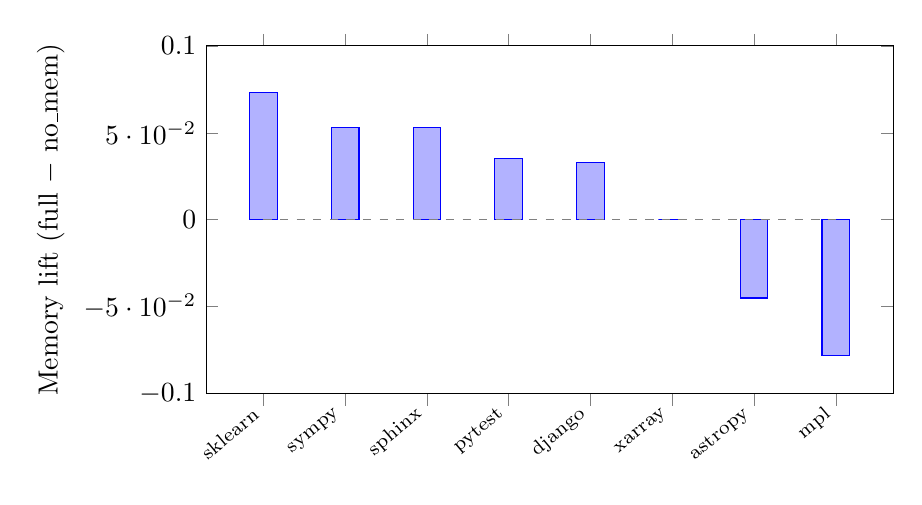
\begin{tikzpicture}\begin{axis}[width=0.85\textwidth,height=6cm,ybar,bar width=10pt,ylabel={Memory lift (full $-$ no\_mem)},
  symbolic x coords={sklearn,sympy,sphinx,pytest,django,xarray,astropy,mpl},xtick=data,
  x tick label style={rotate=40,anchor=east,font=\scriptsize},ymin=-0.10,ymax=0.10]
\addplot coordinates {(sklearn,0.073)(sympy,0.053)(sphinx,0.053)(pytest,0.035)(django,0.033)(xarray,0.000)(astropy,-0.045)(mpl,-0.078)};
\draw[gray,dashed](axis cs:sklearn,0)--(axis cs:mpl,0);
\end{axis}\end{tikzpicture}
\caption{Per-sequence memory lift. Memory helps scikit-learn/sympy/sphinx, hurts
matplotlib/astropy, and does not track structural overlap.}\label{fig:memory-lift}
\end{figure}

\noindent The per-sequence dependency fractions in Table~\ref{tab:memory-lift} are the same
benchmark-structural quantities charted in Figure~\ref{fig:interdependence}; here they serve
as the structural covariate against which the lifts are read.

\subsection{A two-filter account of the bounded benefit}

The lift decomposition and the task-level model below combine into a two-filter explanation
of why the aggregate memory benefit is small even though stored experience is occasionally
decisive. The \emph{first filter} is interdependence: only a minority of tasks
($\approx 0.3$ mean fraction) structurally depend on a predecessor, so by construction memory
cannot help the file-disjoint majority. The \emph{second filter} is utilization: even when a
dependency is present, memory rarely flips the outcome --- the per-sequence lifts are
heterogeneous and frequently negative, and the task-level model (below) finds no policy
effect once difficulty and sequence position are accounted for. The two filters together
shrink a mechanism that is real on specific tasks into an aggregate benefit that the $N=8$
design cannot resolve from zero.

\subsection{Task-level model: position, not policy, governs resolution}

The task-level analysis is a generalized linear mixed model with a binomial/logit link
(Invariant~\#14), fit over all $4{,}914$ task observations with a crossed random effect on
\texttt{task\_id} and \texttt{cls\_consolidation} as the reference policy
(\texttt{glmm\_results.json}; converged). The model isolates the two questions the aggregate
means cannot: whether any policy shifts the per-task odds of resolution once task difficulty
and within-sequence position are controlled, and which covariates actually move the outcome.

No policy coefficient is significant: relative to \texttt{cls\_consolidation},
\texttt{full\_memory} is $+0.116 \pm 0.118$, \texttt{no\_memory} $-0.133 \pm 0.117$,
\texttt{random\_prune} $+0.033 \pm 0.117$, \texttt{recency\_prune} $-0.092 \pm 0.117$, and
\texttt{type\_aware\_decay} $-0.188 \pm 0.117$ --- every one within $2 \times \mathrm{SE}$ of
zero. The policy-null of the sequence-level Wilcoxon (Section~\ref{sec:h1}) therefore holds
at the task level too.

What does move the outcome are the two non-policy covariates. Task difficulty is strongly
negative ($-2.18 \pm 0.065$), as expected, and so is within-sequence position
($-1.49 \pm 0.086$): agent effectiveness \emph{declines across sequence position regardless
of policy}. This is the structural counterpart of the lift result. The agent gets worse as a
sequence progresses --- a trajectory/context-dilution effect --- and crucially, accumulating
memory does \emph{not} rescue it; \texttt{full\_memory}'s task-level odds are statistically
indistinguishable from \texttt{no\_memory}'s. Forgetting is not the cause of late-sequence
decline, and remembering is not its cure.

We report this model on its signs and the null rather than on precise pairwise inference: the
fit is approximate (statsmodels variational estimation; the canonical \texttt{R}/\texttt{lme4}
Laplace fit was not run), and a sensitivity check confirms the direction of the difficulty and
position effects. We do not recompute the untested full-versus-no-memory contrast from the
policy coefficients --- that comparison is the sequence-level Wilcoxon of
Section~\ref{sec:h1}, and reading it off the GLMM coefficients would be test-switching
(Invariant~\#11).

\subsection{Feature analysis: collinearity check passed, helpful/harmful labels deferred}

The pre-registered feature analysis (Invariant~\#13) asks which properties of a retrieved
memory item predict whether it helped or harmed the task it was injected into. The
collinearity prerequisite is satisfied: across $18{,}675$ task--memory pairs the variance
inflation factors are all well below the conventional threshold of $5$ ---
\texttt{semantic\_similarity} $1.42$, \texttt{retrieval\_rank} $1.40$, and
\texttt{memory\_age} $1.02$ --- so the candidate predictors are not redundantly entangled and
a PR-AUC classifier over them would be interpretable.

The classifier itself is deferred. The Tier-1 weak labels available from the run logs are
all-neutral (zero positive instances of the helpful/harmful class), which provides no signal
for a PR-AUC model. Producing the classifier requires Tier-2 manually adjudicated gold
labels, which is downstream work and not a blocker for the headline: the helpful/harmful
prediction would refine \emph{why} a given item helps, but the question of \emph{whether}
memory helps in aggregate is already answered by the lift decomposition and the GLMM above.

\subsection{The anchor-probe sub-study}
\label{sec:a5}

The resolution-rate CL-F1 used throughout this chapter is a proxy; it does not directly
measure continual-learning forgetting or backward retention, and the natural-regime stability
instrument saturates near $1.000$ (Section~\ref{sec:instrument}). To test whether that
saturation reflects genuine robustness or measurement-insensitivity, we ran a separate
construct-validity sub-study --- the A5 anchor probe --- that deliberately constructs cells
where \texttt{full\_memory} retains and retrieves a memory item that a capped pruner has
already evicted. That sub-study is reported as a stand-alone construct-validity analysis and
revisited in the threats-to-validity discussion; it is not part of the H5 task-level model and
does not change the policy-null reported here.

\subsection{Summary}

H5 is, on its surface, a near-null: the aggregate memory benefit is $+1.6$\,pp and
unresolvable from zero. Decomposed, the null is mechanistic rather than empty. Memory helps a
specific minority of sequences, hurts others, and does not track structural overlap; the
benefit it confers is gated by a first filter of interdependence ($\approx 0.3$ of tasks) and
a second filter of utilization (the GLMM policy-null). And the dominant driver of late-sequence
failure --- declining effectiveness with sequence position --- is untouched by how much an
agent remembers. ``Not every task needs memory'' is not a hedge; on this benchmark it is a
measured property, and it is why proactive forgetting is footprint-free on the value axis.

% Generated from the matching Typst scaffold by
% scripts/migrate_typst_report_to_latex.py.

% ── 5.7  Manipulation Checks ─────────────────────────────────────────────
% PURPOSE: Prove the storage manipulation actually reaches the prompt before any outcome
%          is interpreted — the experiment must be visible at the point of injection.
% MOVE: Pain → Consequence → Gap (a manipulation you can't see is a confound you can't rule out).
% FIGURES/TABLES: none.
% CITATIONS: none new.
% ─────────────────────────────────────────────────────────────────────────

\section{Manipulation Checks}
\label{sec:manipulation-checks}

The hypothesis tests in Sections~\ref{sec:h1}--\ref{sec:h5} are only interpretable
if three things actually held during execution: the pruning policies genuinely
discarded memory, every condition retrieved through the same scoring path, and the
underlying model and embedder never moved. A manipulation that cannot be seen at the
point of injection is a confound that cannot be ruled out. This section is therefore
the gate the reader must pass through before reading the preceding results causally:
it confirms that the six policies materially differ in what reaches the prompt, that
they differ \emph{only} in the dimension the design intends, and that the recorded
matrix is internally complete. Throughout, the model is held constant at
\texttt{deepseek-v4-flash} (Deviation~D1), so any between-policy difference cannot be
attributed to a moving generator.

\subsection{The pruning manipulation binds}

The first check is that eviction was not vacuous. The per-policy cap is fixed at
$10$ memory items, whereas every SWE-Bench-CL sequence contains far more tasks than
that: the full matrix comprises $4{,}914$ task rows across $8$ sequences, $3$ seeds
and $6$ policies, so each sequence runs many times longer than the cap. The store
therefore overflows the cap well before any sequence completes, and the pruning
policies are forced to make eviction decisions on every subsequent task rather than
sitting idle. The cap binds by construction.

The clearest \emph{quantitative} evidence that the manipulation reaches the prompt is
the realised memory footprint --- the number of memory tokens actually injected per
task, measured at the point of injection rather than inferred from the store. The
policies separate sharply on this axis:

\begin{itemize}
  \item \texttt{full\_memory} injects \textbf{1{,}247} tokens per task --- it carries
        the whole accumulated store;
  \item the four bounded policies inject roughly half as much ---
        \texttt{cls\_consolidation} \textbf{704}, \texttt{recency\_prune}
        \textbf{604}, \texttt{random\_prune} \textbf{601} and
        \texttt{type\_aware\_decay} \textbf{598} tokens per task --- consistent with a
        store held to the cap rather than allowed to grow;
  \item \texttt{no\_memory} injects \textbf{0} tokens, the clean zero-footprint
        boundary condition.
\end{itemize}

A roughly $2\times$ spread between \texttt{full\_memory} and the pruners, and an exact
zero for \texttt{no\_memory}, demonstrate that the policies change \emph{what lands in
the prompt}, not merely what sits in the store. This footprint separation is reported
here purely as a manipulation check --- evidence that the intervention took effect; its
performance consequences (the footprint axis of H1b) are interpreted in
Section~\ref{sec:h1}, not here.

\subsection{Retrieval is identical across policies}

The second check is that the policies differ \emph{only} in eviction. Retrieval
scoring is pure cosine similarity routed through a single shared code path
(\texttt{shared\_retrieve}, Invariant~\#5): no policy adds bonuses, penalties, or
re-ranking. The same embedder (\texttt{nomic-embed-text-v2-moe}, $768$-d,
Deviation~D2) and the same injection ordering --- relevance-sorted with the best item
placed last to mitigate lost-in-the-middle effects (Invariant~\#6) --- are used in
every condition. Consequently the only thing that varies between the six conditions is
\emph{which items survive in the store to be scored}, which is exactly the
manipulation under test. \texttt{no\_memory} is the degenerate case of this same path
with an empty store: it retrieves nothing by construction, giving a clean lower
boundary that no other condition can leak into. The memory-type classifier (D4) is
run identically across all six conditions and its failures are handled the same way in
each, so it cannot differentially bias any single policy.

\subsection{The full matrix audits clean}

The final check is that the recorded matrix is internally consistent before any
statistic is computed on it. A deep audit of the trustworthy run
(\texttt{runs\_144\_seq\_cceb325}, agent frozen at commit \texttt{cceb325}) returned
\textbf{zero flags} across all $4{,}914$ task rows, of which $2{,}175$ ($44.3\%$) were
resolved. The audit confirmed in particular that:

\begin{itemize}
  \item \textbf{Exact task-id sets.} Every policy and seed was evaluated on the
        identical set of tasks --- no condition received an easier or smaller subset,
        which is itself a manipulation check against selection differences across
        arms.
  \item \textbf{Frozen agent.} The coding agent was pinned at commit
        \texttt{cceb325} for the entire run; \texttt{git diff cceb325..HEAD --
        src/agents} is empty, so the agent code is provably constant across all $144$
        units.
  \item \textbf{Tool-mode consistency.} The per-row tool-mode mismatch that affected
        an earlier matrix was gated and blocked before this run, so no row mixes
        tool-calling conventions.
\end{itemize}

For full transparency, two execution facts are disclosed even though neither affects
the science. First, the orchestration code changed during the run, but only for
disk management --- a per-task \texttt{docker rmi} cleanup gated behind the
\texttt{CLEANUP\_TASK\_IMAGES} environment flag (covered by
\texttt{tests/test\_cleanup\_task\_image.py}); the agent, memory, and evaluation paths
were untouched. Second, one cell (\texttt{random\_prune\_matplotlib\_seed2}) had its
\texttt{RUN\_COMPLETED} marker written by hand \emph{after}
\texttt{validate\_run\_complete} had already passed on its data: the marker file was
lost to a process kill, the underlying outputs are complete, and the hand-written
marker only re-records a completion that the validator had independently confirmed.

\subsection{Provenance}

Each unit's manipulation is auditable after the fact: the model
(\texttt{deepseek-v4-flash}), embedder, seed, cap, and policy configuration are
recorded per run, with model provenance fixed through the run directory plus the
frozen \texttt{base.yaml} and \texttt{MODEL\_PROVENANCE.json}. Taken together, these
checks establish the precondition for reading Sections~\ref{sec:h1}--\ref{sec:h5}
causally: the manipulation is real and visible at the prompt, the conditions differ
only in eviction, and the matrix on which every statistic is computed is complete and
flag-free.


\chapter{Discussion}\label{ch:discussion}
% Generated from the matching Typst scaffold by
% scripts/migrate_typst_report_to_latex.py.

% ── 6.1  Key Findings ────────────────────────────────────────────────────
% PURPOSE: Restate the thesis-defining result up front before any interpretation.
% MOVE: Counter-intuitive lead ("Contrary to the assumption that more memory helps…").
% BEATS: see ordered bullets below — the honest story, ending on the footprint win.
% FIGURES/TABLES: forward-refs fig:pareto-footprint, fig:pareto-compute, tab:main-results (defined in Ch.5).
% CITATIONS: liu2024 (context dilution / Lost-in-the-Middle), xiong2025 (experience-following risk).
% SOURCE-DOC: README grounded-facts cheat sheet; docs/defense-qa.md (Q5).
% ─────────────────────────────────────────────────────────────────────────

\section{Key Findings}

The intuition this thesis set out to test is that more memory should help: an agent
that carries the full record of every task it has solved ought to resolve subsequent
tasks more reliably than one that forgets, and a policy that forgets aggressively ought
to pay for that thrift in lost performance. The trustworthy $144$-run matrix
(\texttt{runs\_144\_seq\_cceb325}, \texttt{deepseek-v4-flash}: $4{,}914$ task rows,
$2{,}175$ resolved, $44.3\%$ overall) does not bear this out. With retrieval held
identical across all six conditions (Invariant~\#5), the value-axis differences between
remembering everything, remembering nothing, and the four forgetting policies are small
enough to be statistically indistinguishable, while the cost of remembering everything is
real and one-sided. The headline is therefore not that forgetting \emph{recovers} lost
performance --- it does not --- but that forgetting is \emph{non-inferior} to full
accumulation on task resolution at roughly half the carried footprint, and that the slow
decline of agent effectiveness across a sequence is driven by something memory
accumulation cannot fix. We restate the five findings here before interpreting them; the
underlying tests are reported in Chapter~\ref{ch:results} (the H1 contrasts in
Table~\ref{tab:main-results}, the frontiers in Figures~\ref{fig:pareto-footprint}
and~\ref{fig:pareto-compute}).

\paragraph{A powered null: no policy beats full memory.}
The pre-registered primary test (Wilcoxon signed-rank on $N=8$ sequence means, each
policy against \texttt{full\_memory}, Holm-corrected over the five contrasts; Invariant
\#11) returns no significant difference: every Holm-corrected $p$ equals $1.000$ and every
$95\%$ BCa interval on the paired difference in resolution crosses zero
(Table~\ref{tab:main-results}). The six policy means are tightly clustered, spanning only
$0.427$ (\texttt{type\_aware\_decay}) to $0.449$ (\texttt{cls\_consolidation}), with
\texttt{full\_memory} at $0.445$ sitting mid-pack rather than at the top. This is the
thesis-defining result: across a clean matrix with no audit flags, accumulating the full
memory record neither beats nor is beaten by proactive forgetting on the resolution proxy.

\paragraph{A small, bounded memory benefit that the design cannot resolve.}
The one comparison that speaks to whether memory helps \emph{at all} ---
\texttt{full\_memory} ($0.445$) against \texttt{no\_memory} ($0.429$) --- shows a benefit
of $+1.6$ percentage points on the policy means (a paired median improvement of $+3.4$
points in full memory's favour). The benefit points the expected direction but is small
and statistically indistinguishable from zero (Holm $p = 1.000$, $r_{rb} = -0.286$, BCa
CI on the paired difference crossing zero). We report it as a \emph{bound}, not a power
verdict: the $N=8$ sequence-level design is underpowered for effects of this magnitude, so
the honest reading is that any benefit from carrying memory is, at the resolution proxy's
granularity, no larger than a few percentage points. Non-inferiority is read from these
bounded intervals rather than from a TOST verdict --- TOST was pre-registered but not
computed (Section~\ref{sec:threats}).

\paragraph{Forgetting is footprint-free.}
The efficiency contribution (H1b) splits cleanly across two axes. On the
\emph{footprint} axis --- the memory tokens carried per task, which governs storage and
retrieval-index growth over an agent's lifetime --- the forgetting policies carry $598$ to
$704$ tokens against \texttt{full\_memory}'s $1{,}247$, roughly half the load, while
\texttt{no\_memory} holds the zero-footprint corner (Figure~\ref{fig:pareto-footprint}).
On the \emph{compute} axis the policies barely separate: total tokens per run rise only
from $5.74$M (\texttt{no\_memory}) to $6.09$M (\texttt{full\_memory}), with the five
memory-carrying policies within about $2\%$ of one another and the whole field spanning
roughly $6\%$ (Figure~\ref{fig:pareto-compute}); tool-call counts are essentially flat at
$\sim\!21$ for every policy. The reason is structural: cost is dominated by the agent loop,
whose growing conversation is resent at each of up to $20$ ReAct steps, so the memory
payload is a small fraction of the per-task token bill. Pruning therefore buys a bounded
footprint --- the quantity that matters for a long-lived agent --- essentially for free,
without sacrificing resolution and without reducing compute. This is the most robust
positive result in the thesis.

\paragraph{Performance declines along the sequence regardless of policy.}
The task-level GLMM (binomial/logit with crossed random effects on task identity;
Invariant~\#14; $4{,}914$ observations) locates the dominant source of variance not in the
memory policy but in the task: the coefficients for difficulty ($-2.18 \pm 0.065$) and for
position within the sequence ($-1.49 \pm 0.086$) are large and significant, whereas every
policy coefficient is smaller than twice its standard error (e.g.\ \texttt{full\_memory}
$+0.116 \pm 0.118$, \texttt{no\_memory} $-0.133 \pm 0.117$). Agent effectiveness thus
\emph{declines as the agent moves deeper into a sequence}, and accumulating memory does not
arrest that decline --- consistent with the context-dilution mechanism behind the
Lost-in-the-Middle effect \cite{liu2024} rather than with a memory deficit that more
storage could repair. (The GLMM is fit by an approximate variational routine rather than
the canonical \texttt{lme4} estimator; we report signs and the policy-null, and a
sensitivity check confirms the direction.)

\paragraph{When forgetting is mis-specified, it can underperform carrying no memory.}
The finding that most sharpens the story is descriptive but mechanistically clear.
\texttt{type\_aware\_decay} posts the \emph{lowest} mean of all six policies ($0.427$),
fractionally below even \texttt{no\_memory} ($0.429$), and it carries the
largest-magnitude effect of the five contrasts ($r_{rb} = -0.444$) --- yet that contrast
remains non-significant after Holm correction ($p = 1.000$), so this is an ordering and a
mechanism, not a statistically established loss. The mechanism is concrete: in the frozen
decay formula the retrieval-frequency term $(1 + \texttt{use\_count})^{0.5}$ dominates the
age-decay term, so a handful of early, high-use memories become effectively permanent
while newer items are evicted almost immediately. A content audit confirms the store
freezes at roughly its first ten items. A forgetting policy that keeps the wrong things can
thus do marginally worse than keeping nothing --- a cautionary result about
\emph{specification}, not about forgetting in general, and a concrete instance of the
experience-following risk \cite{xiong2025}.

\paragraph{The frame.}
Taken together, these findings replace the expected ``more memory helps'' narrative with a
more precise one. On the resolution proxy, forgetting is non-inferior to full accumulation
at materially lower footprint and no compute penalty; the reason the average memory benefit
is so small is structural --- only a minority of tasks (a mean dependency fraction of
$\sim\!0.3$) actually depend on a predecessor, so most of the matrix has no continual-
learning signal for memory to exploit, and even where dependency exists the benefit is
heterogeneous (Section~\ref{sec:h5}). The contribution is therefore not that forgetting
recovers performance, but that it costs nothing to forget here, and that quantifying
\emph{when} memory could matter --- interdependence as the binding filter --- is where the
continual-learning question actually lives. Throughout, we read these results against the
proxy's known limit: CL-F1 is an end-of-sequence \emph{resolved-rate} proxy, not a
fine-grained forgetting curve, a gap we probe directly in the A5 anchor sub-study and
revisit under construct validity (Section~\ref{sec:threats}).

% Generated from the matching Typst scaffold by
% scripts/migrate_typst_report_to_latex.py.

% ── 6.2  Interpretation and Implications ─────────────────────────────────
% PURPOSE: Turn the key findings into "when to forget", practitioner guidance, theory.
% MOVE: Pivot ("Rather than treat memory as always-on, treat forgetting as dosage").
% BEATS: see ordered bullets below — dosage → practitioner guidance → theory.
% FIGURES/TABLES: fig:interdependence (memory-lift by position + ~⅓ overlap).
% CITATIONS: xiong2025; anderson1991, richards2017 (transience as adaptive).
% SOURCE-DOC: README grounded-facts; docs/defense-qa.md (Q5).
% ─────────────────────────────────────────────────────────────────────────

\section{Interpretation and Implications}

\subsection{From always-on memory to footprint-free forgetting}

The dominant assumption in agent-memory engineering is that retention is an
unalloyed good: store every solved task, retrieve what is similar, and let the
accumulated experience compound. Our results invite a different default. With
retrieval held constant across all six policies (Invariant~\#5), no forgetting
policy is distinguishable from \texttt{full\_memory} on the CL-F1 resolve-rate
proxy --- every one of the five pre-registered Wilcoxon contrasts is
non-significant after Holm correction, and every rank-biserial effect carries a
bootstrap confidence interval that crosses zero. The benefit of unbounded
accumulation over carrying no memory at all is small (a $+1.6$~pp difference in
means, $0.445$ versus $0.429$; paired median $\Delta \approx +3.4$~pp) and itself
non-significant; the $N=8$ sequence-level design cannot resolve effects of this
magnitude, so we report it as a bounded benefit rather than a confirmed one.

What \emph{does} separate the policies is footprint. \texttt{full\_memory} carries
roughly $1{,}247$ tokens of injected context per task; the pruners carry between
$\sim\!600$ and $\sim\!700$ --- about half --- while \texttt{no\_memory} occupies
the zero-footprint corner (\Cref{fig:pareto-footprint}). Crucially, this saving is
\emph{not} a saving on compute: total tokens per run vary only from $5.74$M
(\texttt{no\_memory}) to $6.09$M (\texttt{full\_memory}), the five memory-carrying
policies fall within $\sim\!2\%$ of one another, and tool-call counts sit at
$\sim\!21$ for every policy. Cost in this agent is dominated by the
reasoning--action loop, not by the memory payload (\Cref{fig:pareto-compute}). The
practical implication reframes the question. Forgetting is not a lever that
recovers lost performance, nor a way to spend less compute; it is a way to keep the
injected context \emph{bounded at no measurable cost to the outcome}. Forgetting,
on this evidence, is close to free --- and ``free'' is precisely why it should be
the default rather than the exception.

\subsection{Dosage: target memory at the interdependent minority}

If accumulation is not what helps, the useful question is no longer ``store
everything or nothing'' but \emph{dosage}: how much memory, aimed at which tasks.
The mechanism behind the diluted average makes this concrete. Only a minority of
tasks structurally depend on a predecessor --- across the eight sequences the
fraction of tasks whose gold-patch files overlap an earlier task averages
$\sim\!0.3$, and ranges from $0.13$ (scikit-learn) to $0.57$ (pydata/xarray)
(\Cref{fig:interdependence}). This is a property of the benchmark, not of any
policy. For the file-disjoint majority, prior memory has nothing relevant to
contribute, so even a perfect retention policy is averaged against a large
population of tasks it cannot affect. ``Not every task needs memory'' is, on these
data, a measurable structural fact rather than a slogan.

Interdependence is necessary but not sufficient. Per-sequence memory lift (full
minus no-memory resolve rate) does \emph{not} track structural overlap: scikit-learn
has the lowest dependency ($0.13$) yet the highest lift ($+0.073$), while xarray has
the highest dependency ($0.57$) yet essentially zero lift, and matplotlib and
astropy show negative lift (\Cref{fig:memory-lift}). A dependency must additionally
be retrievable and the retrieved item must actually be used before it can flip an
outcome --- a chain of filters, each of which loses tasks. Forgetting is the
mechanism that realizes the dosage: by keeping memory small it concentrates the
limited retrieval budget on the few items most likely to matter, without paying the
footprint of carrying the rest. The contribution here is less a winning policy than
the quantification of \emph{why} the average benefit is small.

\subsection{Practitioner guidance}

Three recommendations follow directly. First, a \emph{simple bounded pruner is the
safe default}. A small memory budget (we used a cap of ten items) combined with a
content-agnostic eviction rule --- random or recency --- matches full accumulation
on the proxy at roughly half the footprint and at no compute penalty. There is no
reason to pay for unbounded storage growth that does not recover performance, and on
largely file-disjoint task streams an aggressive pruner is non-inferior; richer
retention should be reserved for repositories with demonstrably high task
interdependence.

Second, \emph{do not pay for content-awareness}. Neither content-aware policy beat
random pruning: CLS consolidation ($0.449$) is statistically indistinguishable from
random ($0.447$), and Type-Aware Decay is the lowest-scoring policy of all six
($0.427$). There is no evidence in these results that inspecting memory content to
decide what to keep buys anything over discarding items blindly.

Third, and most concretely, \emph{avoid pure retrieval-frequency decay} --- the
Type-Aware Decay trap. Its formal Wilcoxon contrast does not reach significance
(Holm $p = 1.000$), so this is a mechanistic caution rather than a measured loss,
but the warning signs converge: TAD carries the largest negative effect of any
policy (medium, $r_{rb} = -0.444$) and is the only policy whose mean falls below
\texttt{no\_memory}. The cause is structural. The retrieval-count term
$(1+\text{use\_count})^{0.5}$ in the decay formula (Invariant~\#8) overwhelms the
age term: early, high-use memories become effectively permanent while newly written
items are evicted almost immediately, so the store freezes at its first
$\sim\!10$ items and stops adapting. A decay rule that rewards past retrieval can
thus entrench stale experience --- precisely the experience-following risk
identified by \cite{xiong2025} --- and should be avoided in favour of simpler
bounded eviction.

\subsection{Where the field should look next}

The strongest forward-looking signal in our data is not about storage policy at all.
The task-level GLMM (Invariant~\#14) finds that none of the policy coefficients
reach significance, but two factors do: task difficulty and, decisively, sequence
position (coefficient $-1.49 \pm 0.086$). Agent effectiveness declines as a sequence
progresses regardless of which memory policy is in force, and accumulating memory
does not rescue it. This points away from eviction policy as the productive frontier
and toward the retrieval and trajectory pathway --- the position-dependent decline
that resembles context dilution rather than a failure of what to remember. If the
field wants to improve continual performance, the leverage appears to lie in how
relevant experience is surfaced and woven into a long trajectory, and in the
structure of task interdependence itself, not in the choice of forgetting rule. The
storage-policy question, at least under a held-constant retriever on this benchmark,
is largely settled in the negative; the retrieval-and-position question is open.

\subsection{Theoretical implication: transience as adaptive}

These findings sit comfortably with a long-standing view in cognitive science that
forgetting is not a defect of memory but a feature of it. The rational analysis of
memory holds that the decay of an item's availability tracks the declining
probability that it will be needed, so transience is an adaptation to the statistics
of the environment rather than a leak \cite{anderson1991}; more recent work argues
that active forgetting promotes generalisation and flexible behaviour rather than
degrading it \cite{richards2017}. Our footprint-non-inferiority result is the
engineering analogue: an agent that proactively discards most of its past pays no
measurable outcome penalty, because most of that past was never going to be
retrieved or used. Bounded, forgetful memory is not a compromise forced by resource
limits; on a task stream where only a minority of items remain relevant, it is the
rational policy.

% Generated from the matching Typst scaffold by
% scripts/migrate_typst_report_to_latex.py.

% ── 6.3  Deviations from Pre-Registration ────────────────────────────────
% PURPOSE: Disclose every deviation (D1–D6) and amendment (A1–A7) as the paper trail
%          that protects the study against "you moved the goalposts after seeing data".
% MOVE: Limitation → Root cause → Trade-off → Connect (the principled-amendment framing).
% BEATS: see ordered bullets below — D-chain, A-chain, then the four-part defense.
% FIGURES/TABLES: tab:deviations (D1–D6, A1–A7 summary).
% CITATIONS: none new.
% SOURCE-DOC: AMENDMENTS.md (authoritative); CLAUDE.md deviation table; defense-qa Q10.
% ─────────────────────────────────────────────────────────────────────────

\section{Deviations from Pre-Registration}
\label{sec:deviations}

\begin{todobox}
Expand the beats below into prose. Point the reader to tab:deviations for the full list; in text, foreground the PRINCIPLED-AMENDMENT framing. Stress each entry is dated, justified, held constant across conditions, and decided BEFORE the affected data --- not p-hacking. Pre-registration is THESIS\_FINAL\_v5.
\end{todobox}

% - DEVIATIONS D1–D6 (runtime): D1 model GPT-5.4 → Kimi-k2.6 → MiniMax M3; D2 embedder →
%   local nomic-embed-text-v2-moe (768-d); D3 cost metric → token-count proxy (flat-rate
%   provider); D4 classifier → JSON-mode + Pydantic; D5 host → x86_64 DigitalOcean droplet
%   + 5-VPS fleet; D6 M3 specifics — reasoning/CoT stripped (D6a), no JSON mode → tolerant
%   extraction (D6b), 16-key rotation failing-closed (D6c). See tab:deviations.
% - AMENDMENTS A1–A7 (pre-registration): A1 record cap 100 → 10 (makes pruning bind on all
%   8 sequences, H2 testable); A2 temperature 0 → 1 (endpoint rejects 0); A3 CLS old-memory
%   threshold 10 → 5 (= cap/2); A4 H1b reframed token-savings → footprint + retrieval
%   latency; A5 anchor-probe scope (PENDING — see §6.4 / docs/a5-anchor-probe-decision.md);
%   A6 seeds 3 → 1 (WITHDRAWN); A7 3 seeds / 144 runs RESTORED (free-unlimited provider + fleet).
% - THE PRINCIPLED-AMENDMENT FRAME (the four-part test, every entry passes): each change is
%   (a) a mechanical fix to an inconsistency a deviation introduced OR a construct correction
%   the mechanism demands; (b) dated and decided BEFORE the affected data is collected;
%   (c) held constant across all conditions × seeds (a fixed factor — contrasts stay valid);
%   (d) disclosed here. This is the line between principled amendment and researcher-DoF abuse.
% - Absolute solve rates are explicitly NOT comparable to GPT-5.4 / SWE-Bench leaderboards;
%   only between-policy contrasts on the fixed model are claimed.

% Generated from the matching Typst scaffold by
% scripts/migrate_typst_report_to_latex.py.

% ── 6.4  Threats to Validity ─────────────────────────────────────────────
% PURPOSE: Reframe the study's limits as conscious trade-offs across the four validity types.
% MOVE: Limitation → Root cause → Trade-off → Connect (per the storytelling template).
% BEATS: see ordered bullets below — construct/measurement, internal, external, statistical.
% FIGURES/TABLES: none (cross-ref tab:deviations from 6.3).
% CITATIONS: SWE-Bench-Illusion 2506.12286 [VERIFY+ADD], Phi-4-reasoning 2504.21318
%   [VERIFY+ADD], Non-Determinism 2408.04667 [VERIFY+ADD]; xiong2025.
% SOURCE-DOC: docs/threats-to-validity.md (prose); docs/a5-anchor-probe-decision.md (probe).
% ─────────────────────────────────────────────────────────────────────────

\section{Threats to Validity}
\label{sec:threats}

\begin{todobox}
Expand the beats below into prose using LIMITATION \textrightarrow{} ROOT CAUSE \textrightarrow{} TRADE-OFF \textrightarrow{} CONNECT for each. Prose is largely drop-in from docs/threats-to-validity.md. Group under the four validity headings. Thread "footprint" and "not every task needs memory".
\end{todobox}

% - CONSTRUCT & MEASUREMENT: anchor-probe stability saturated at 1.000 on the 5-anchor
%   gate-3 sample — may be instrument INSENSITIVITY (this is the E7 interdependence
%   phenomenon: anchors drawn from the file-disjoint ⅔ cannot move) rather than true
%   absence of forgetting; tested under A5 (docs/a5-anchor-probe-decision.md). Cost axis
%   inflated by M3 reasoning tokens [VERIFY+ADD] (Phi-4-reasoning 2504.21318) — uniform
%   across conditions, so contrasts hold, absolute not comparable. CLS inert (0 clusters)
%   → H3 reported N/A, not supported; declined to relax the frozen 0.70 threshold.
% - INTERNAL: contamination (SWE-Bench public, M3 cutoff undocumented) is CONSTANT across
%   conditions → biases absolute solve rates, NOT between-policy contrasts [VERIFY+ADD]
%   (SWE-Bench-Illusion 2506.12286); per-run provenance (model alias, config hash, dataset
%   revision) logged to detect router/alias drift.
% - EXTERNAL: single base model (M3, third link of declared D1 chain) — a SCOPE BOUNDARY
%   defended by scope + cost-axis cleanliness + bandwidth, NOT budget (free-unlimited
%   provider + 5-VPS fleet removed compute as a constraint); same-repo retrieval only;
%   fixed top_k=5. Deeper bound: only ~⅓ of tasks are interdependent, so "memory helps"
%   claims apply to that subset, not sequential coding in general @xiong2025.
% - STATISTICAL-CONCLUSION: N=8 sequence-level means is honestly underpowered for small
%   effects → LEAD WITH ESTIMATION (effect sizes + BCa intervals) over dichotomous
%   significance; run-level seed variance reported SEPARATELY from task-level bootstrap,
%   never pooled (two distinct variance sources) [VERIFY+ADD] (Non-Determinism 2408.04667).


\chapter{Conclusion and Future Work}\label{ch:conclusion}
% Generated from the matching Typst scaffold by
% scripts/migrate_typst_report_to_latex.py.

% ── 7.1  Conclusion ──────────────────────────────────────────────────────
% PURPOSE: Restate the thesis and recap the metric → trade-off in one tight pass.
% MOVE: Restate + metric → trade-off recap (per the storytelling template).
% BEATS: see ordered bullets below — what we measured, the result, the reframe, the contribution.
% FIGURES/TABLES: none (cross-ref fig:pareto-footprint from Ch5/6).
% CITATIONS: none new (xiong2025 if interdependence is cited).
% SOURCE-DOC: README grounded-facts; docs/defense-qa.md (Q5).
% ─────────────────────────────────────────────────────────────────────────

\section{Conclusion}

\begin{todobox}
Expand the beats below into prose. RESTATE the study, recap the metric \textrightarrow{} trade-off, end by naming the contribution as a template, not a new policy. Thread "retrieval held constant", "non-inferiority", "footprint", "not every task needs memory". Numbers stay placeholders --- full 144-run matrix still RUNNING.
\end{todobox}

% - RESTATE: this thesis is a controlled measurement of six forgetting policies for AI
%   coding agents on SWE-Bench-CL, with retrieval held constant (pure cosine, identical
%   across all six) so the storage/forgetting policy is the only moving part.
% - METRIC → TRADE-OFF RECAP: on CL-F1, forgetting is non-inferior to full-memory
%   accumulation [RESULT: TOST, SESOI ±0.03] at materially lower memory footprint
%   [RESULT: …] — the footprint axis (A4) is where forgetting wins.
% - THE REFRAME: because only ~⅓ of tasks are interdependent [RESULT: ~0.30 overlap /
%   ~0.32 frac], memory is best understood as a DOSAGE / TARGETING question — "not every
%   task needs memory" — rather than an always-on accumulation default.
% - THE CONTRIBUTION: a clean, reproducible experimental TEMPLATE (retrieval-fixed
%   isolation, No-Memory↔Full-Memory bracketing, two-axis Pareto, interdependence
%   quantification, 144-run artifact) — NOT a new memory policy.

% Generated from the matching Typst scaffold by
% scripts/migrate_typst_report_to_latex.py.

% ── 7.2  Future Work ─────────────────────────────────────────────────────
% PURPOSE: Each future item traces a NAMED limitation from §6.4 to a concrete next study.
% MOVE: Future-work-per-bottleneck (each item closes a named threat to validity).
% BEATS: see ordered bullets below — cross-model · anchor-probe · decontamination · cross-repo.
% FIGURES/TABLES: none.
% CITATIONS: SWE-rebench 2505.20411 [VERIFY+ADD], SWE-MERA 2507.11059 [VERIFY+ADD].
% SOURCE-DOC: docs/threats-to-validity.md; docs/a5-anchor-probe-decision.md; AMENDMENTS (D-0.4).
% ─────────────────────────────────────────────────────────────────────────

\section{Future Work}

\begin{todobox}
Expand the beats below into prose. Each item must NAME the §6.4 limitation it addresses, then propose the concrete next study. Keep the single-model and same-repo scope honest; frame these as follow-ups, not weaknesses of the present design.
\end{todobox}

% - CROSS-MODEL PROBE (addresses single-model external validity, §6.4): the D-0.4
%   descriptive 12-run probe — top conditions × a subset of sequences × one seed — to
%   report transfer DIRECTION only (non-inferential), not a generalization claim.
% - ANCHOR-PROBE SENSITIVITY TEST (addresses stability = 1.000, §6.4 construct threat):
%   the A5 discrimination test — target anchors at INTERDEPENDENT tasks (gold-patch files
%   overlapping a later task) on a high-overlap sequence, run Full vs aggressive-prune ≥3×,
%   check whether stability ever discriminates before committing the full-probe budget.
% - DECONTAMINATED BENCHMARKS (addresses contamination, §6.4 internal threat): re-run on
%   SWE-rebench (2505.20411) [VERIFY+ADD] / SWE-MERA (2507.11059) [VERIFY+ADD] — post-cutoff,
%   continuously-refreshed task streams — to recover interpretable ABSOLUTE solve rates.
% - CROSS-REPO RETRIEVAL (addresses same-repo scope, §6.4 external threat): relax the
%   same-repo-only invariant to test whether forgetting policies transfer when memory is
%   drawn across repositories, where interdependence structure differs.


\appendix
\chapter{Appendices}\label{ch:appendix}
% Generated from the matching Typst scaffold by
% scripts/migrate_typst_report_to_latex.py.

% ── Appendix A  Reproducibility and Provenance ───────────────────────────
% PURPOSE: Give a reader everything needed to reproduce the matrix and audit provenance.
% MOVE: none (reference appendix — structured disclosure, not narrative).
% BEATS: see ordered bullets below — pre-reg, archive, seeds, environment, model, logging, reversibility.
% FIGURES/TABLES: cross-ref tab:deviations (§6.3).
% CITATIONS: none new.
% SOURCE-DOC: AMENDMENTS.md (D2/D5/D6); CLAUDE.md (provider config, logging schemas v5 §11).
% ─────────────────────────────────────────────────────────────────────────

\section{Reproducibility and Provenance}
\label{sec:reproducibility}

This appendix lists what a replicator needs to re-derive the matrix and audit its provenance.
Each item names the concrete artifact to consult. The reported matrix is
\texttt{runs\_144\_seq\_cceb325} (data) analysed into \texttt{results\_seq\_cceb325}
(tables, GLMM, plots); the full deep audit returned $0$ flags.

\begin{description}
  \item[Pre-registration.] The frozen design is \texttt{THESIS\_FINAL\_v5} ($26$ frozen
    decisions, $16$ invariants). Every change from it is logged as a dated deviation or
    amendment (D1--D8, A1--A7) in \texttt{AMENDMENTS.md} and summarised in
    Table~\ref{tab:deviations} (Section~\ref{sec:deviations}).
  \item[Frozen experiment commit.] All $144$ cells were produced by the agent code frozen at
    commit \texttt{cceb325} (\texttt{git diff cceb325..HEAD -- src/agents/} is empty), so the
    science is identical across the matrix. The instrument hotfix that defines \texttt{cceb325}
    is described in Section~\ref{sec:instrument}; orchestration changes made during execution
    (per-task Docker image cleanup, sequence-phased scheduling) are disk-management only and do
    not alter what is computed.
  \item[Design and seeds.] Six policies $\times$ eight official SWE-Bench-CL sequences $\times$
    three seeds $=144$ runs (A7-restored). Seeds are indexed $1$--$3$ and applied identically
    across all policies and sequences; the cell directory names encode policy, sequence, and
    seed (e.g.\ \texttt{cls\_consolidation\_django\_seed2}). The three per-seed CL-F1 values per
    cell are retained in \texttt{aggregated/sequence\_aggregates.json}.
  \item[Model provenance.] The executed model is a single frozen
    \texttt{deepseek-v4-flash} on OpenCode serving \emph{all} roles --- agent, $5$-type
    classifier, reflection, and CLS summariser (D8). It is the endpoint of a disclosed chain of
    OpenAI-compatible substitutions away from the pre-registered GPT-5.4 (Section~\ref{sec:deviations});
    the intermediate MiniMax~M3 run (D6) was discarded with no usable data. Because the model is
    held constant across all conditions, it is a fixed factor; absolute resolution rates are not
    comparable to GPT-5.4 or public leaderboards. A rotating key pool fails closed on quota
    exhaustion so balance depletion is never recorded as a false \texttt{resolved=0}.
  \item[Computational environment.] An x86\_64 cloud fleet with prebuilt SWE-bench instance
    images (D5); embeddings from a local Ollama \texttt{nomic-embed-text-v2-moe} ($768$-d,
    deterministic) (D2); cost recorded as a token-count proxy because the provider is flat-rate
    (D3). Reasoning tokens are stripped deterministically before parsing, embedding, and
    re-injection, so the memory payload is reasoning-free (D6a/D8a).
  \item[Per-run logging.] Each run records its configuration and model identity alongside
    \texttt{task\_results.jsonl}, \texttt{memory\_events.jsonl}, per-task trajectories, and
    before/after memory snapshots (v5~\S11 schemas). These are the inputs the audit and the
    analysis pipeline consume.
  \item[Re-derivation.] The full analysis is reproduced with
    \texttt{python -m scripts.run\_analysis --stage all --runs-dir runs\_144\_seq\_cceb325
    --out results\_seq\_cceb325}; the task-level GLMM is a separate stage
    (\texttt{src.analysis.glmm.run\_task\_level\_analysis}).
  \item[Reversibility.] The provider is selected entirely through \texttt{.env}; chat and
    embedding clients are separate (no global \texttt{OPENAI\_BASE\_URL}), so the model and
    embedder deviations are configuration-only and reversible to GPT-5.4/OpenAI without code
    changes.
\end{description}

% Generated from the matching Typst scaffold by
% scripts/migrate_typst_report_to_latex.py.
% INTEGRITY: all numbers from results_seq_cceb325 (trustworthy 144; deepseek-v4-flash;
% agent frozen cceb325; deep audit 0 flags). No fabricated cells.

% ── Appendix B  Extended Results ─────────────────────────────────────────
% PURPOSE: Host the full-detail per-cell tables and the GLMM specification that would
%          clutter Chapter 5. Tables + one-line explanations, not narrative.
% ─────────────────────────────────────────────────────────────────────────

\section{Extended Results}

This appendix gives the per-cell breakdowns behind the aggregate contrasts of
Chapter~\ref{ch:results} and the full specification of the task-level model. All values are
from the trustworthy 144-run matrix (\texttt{runs\_144\_seq\_cceb325}; deep audit, 0 flags);
the complete per-seed records, trajectories, and memory-event logs are in the released
artifact (Appendix~\ref{sec:reproducibility}).

\subsection{Per-sequence resolution by policy}

Table~\ref{tab:per-sequence} reports CL-F1 (the resolved-rate proxy, mean over three seeds)
for every sequence--policy cell; column $n$ is the number of evaluated tasks in the sequence.
The per-policy means in the final
row are the values carried into the H1 contrasts (Table~\ref{tab:main-results}). The cell-level
view shows how the tight aggregate clustering (means $0.427$--$0.449$) is the average of much
larger, sign-varying per-sequence swings --- e.g.\ \texttt{full\_memory} ranges from $0.284$
(matplotlib) to $0.677$ (scikit-learn) --- which is the heterogeneity dissected in
Section~\ref{sec:h5}.

\begin{table}[htbp]
  \centering
  \caption{CL-F1 (resolved-rate proxy), mean over three seeds, per sequence $\times$ policy.
  Final row is the across-sequence mean (the H1 inputs). \texttt{runs\_144\_seq\_cceb325}.}
  \label{tab:per-sequence}
  \small
  \begin{tabular}{lrrrrrrr}
    \toprule
    Sequence & no\_mem & full & random & recency & TAD & cls & $n$ \\
    \midrule
    scikit-learn & 0.604 & 0.677 & 0.646 & 0.688 & 0.615 & 0.635 & 32 \\
    sympy        & 0.393 & 0.447 & 0.447 & 0.393 & 0.427 & 0.413 & 50 \\
    sphinx       & 0.341 & 0.394 & 0.326 & 0.318 & 0.303 & 0.333 & 44 \\
    pytest       & 0.491 & 0.526 & 0.632 & 0.544 & 0.544 & 0.579 & 19 \\
    django       & 0.560 & 0.593 & 0.567 & 0.547 & 0.553 & 0.573 & 50 \\
    xarray       & 0.318 & 0.318 & 0.333 & 0.379 & 0.333 & 0.439 & 22 \\
    astropy      & 0.364 & 0.318 & 0.303 & 0.288 & 0.333 & 0.333 & 22 \\
    matplotlib   & 0.363 & 0.284 & 0.324 & 0.343 & 0.304 & 0.284 & 34 \\
    \midrule
    \textbf{Mean} & 0.429 & 0.445 & 0.447 & 0.437 & 0.427 & 0.449 & \\
    \bottomrule
  \end{tabular}
\end{table}

\subsection{Per-sequence memory footprint by policy}

Table~\ref{tab:per-sequence-footprint} reports the carried memory footprint (tokens per task,
mean over three seeds) for the same cells. \texttt{no\_memory} is zero by construction; the
pruning policies sit near their $\sim\!600$-token caps across all sequences, while
\texttt{full\_memory}'s footprint grows with sequence length and difficulty (up to $1{,}894$
on sympy). This is the footprint-axis separation of Figure~\ref{fig:pareto-footprint} made
explicit per sequence.

\begin{table}[htbp]
  \centering
  \caption{Memory footprint (tokens/task), mean over three seeds, per sequence $\times$ policy.
  \texttt{runs\_144\_seq\_cceb325}.}
  \label{tab:per-sequence-footprint}
  \small
  \begin{tabular}{lrrrrrr}
    \toprule
    Sequence & no\_mem & full & random & recency & TAD & cls \\
    \midrule
    scikit-learn & 0 & 1063 & 584 & 580 & 559 & 660 \\
    sympy        & 0 & 1894 & 654 & 687 & 644 & 810 \\
    sphinx       & 0 & 1587 & 642 & 642 & 668 & 765 \\
    pytest       & 0 & 799  & 595 & 597 & 588 & 669 \\
    django       & 0 & 1858 & 644 & 679 & 670 & 788 \\
    xarray       & 0 & 786  & 537 & 515 & 509 & 601 \\
    astropy      & 0 & 790  & 566 & 555 & 570 & 634 \\
    matplotlib   & 0 & 1198 & 584 & 578 & 578 & 708 \\
    \bottomrule
  \end{tabular}
\end{table}

\subsection{Task-level GLMM specification and estimates}

Table~\ref{tab:glmm-spec} gives the full fixed- and random-effect estimates for the
binomial/logit GLMM summarised in Section~\ref{sec:h5} (Invariant~\#14). The model is
\[
  \texttt{resolved} \sim \texttt{C(policy)} + \texttt{difficulty} + \texttt{position}
  + (1 \mid \texttt{seq\_seed}) + (1 \mid \texttt{task\_id}),
\]
fit over $4{,}914$ observations in $24$ groups with \texttt{cls\_consolidation} as the
reference policy. The estimator is an approximate variational routine
(\texttt{BinomialBayesMixedGLM}); the canonical \texttt{R}/\texttt{lme4} Laplace fit was not
run, so we report signs and the policy-null rather than exact pairwise inference, and a
random-intercepts-only sensitivity fit reproduces the difficulty and position signs. The large
\texttt{task\_id} random-effect variance ($3.22$) relative to the \texttt{seq\_seed} variance
($0.13$) confirms that most outcome variance is per-task, not per-policy --- the structural
basis of the policy-null.

\begin{table}[htbp]
  \centering
  \caption{GLMM fixed-effect estimates (log-odds) and random-effect variances. No policy
  coefficient exceeds twice its standard error; difficulty and position are large and
  significant. Reference policy = \texttt{cls\_consolidation}. \texttt{glmm\_results.json}.}
  \label{tab:glmm-spec}
  \begin{tabular}{lrr}
    \toprule
    Term & Coef.\ (log-odds) & Std.\ err. \\
    \midrule
    Intercept                          & $+1.144$ & $0.048$ \\
    policy: full\_memory               & $+0.116$ & $0.118$ \\
    policy: no\_memory                 & $-0.133$ & $0.117$ \\
    policy: random\_prune              & $+0.033$ & $0.117$ \\
    policy: recency\_prune             & $-0.092$ & $0.117$ \\
    policy: type\_aware\_decay         & $-0.188$ & $0.117$ \\
    difficulty (numeric)               & $-2.180$ & $0.065$ \\
    position (normalised)              & $-1.491$ & $0.086$ \\
    \midrule
    \multicolumn{3}{l}{\emph{Random-effect variance:}\quad
      \texttt{seq\_seed} $=0.128$,\quad \texttt{task\_id} $=3.223$} \\
    \bottomrule
  \end{tabular}
\end{table}

\subsection{What the released artifact additionally contains}

Beyond these aggregate tables, the run archive retains, per cell: the three per-seed CL-F1
values (\texttt{seed\_cl\_f1\_values} in \texttt{aggregated/sequence\_aggregates.json}),
per-task resolution and patch records (\texttt{task\_results.jsonl}), the full memory-event
stream (writes, evictions, retrievals; \texttt{memory\_events.jsonl}), per-task trajectories,
and before/after memory snapshots. The feature-analysis VIF inputs ($18{,}675$
task--retrieved-memory pairs) and the deferred Tier-2 helpful/harmful labelling slot live under
\texttt{feature\_importance/}. These support re-derivation of every figure and table in
Chapter~\ref{ch:results} via \texttt{scripts/run\_analysis} (Appendix~\ref{sec:reproducibility}).


\backmatter
\nocite{*}
\bibliographystyle{plain}
\bibliography{references}

\end{document}
